%%% Title:    DSS Stats & Methods: Lecture 6
%%% Author:   Kyle M. Lang
%%% Created:  2017-09-12
%%% Modified: 2020-09-18

\documentclass{beamer}\usepackage[]{graphicx}\usepackage[]{color}
% maxwidth is the original width if it is less than linewidth
% otherwise use linewidth (to make sure the graphics do not exceed the margin)
\makeatletter
\def\maxwidth{ %
  \ifdim\Gin@nat@width>\linewidth
    \linewidth
  \else
    \Gin@nat@width
  \fi
}
\makeatother

\definecolor{fgcolor}{rgb}{0, 0, 0}
\newcommand{\hlnum}[1]{\textcolor[rgb]{0.69,0.494,0}{#1}}%
\newcommand{\hlstr}[1]{\textcolor[rgb]{0.749,0.012,0.012}{#1}}%
\newcommand{\hlcom}[1]{\textcolor[rgb]{0.514,0.506,0.514}{\textit{#1}}}%
\newcommand{\hlopt}[1]{\textcolor[rgb]{0,0,0}{#1}}%
\newcommand{\hlstd}[1]{\textcolor[rgb]{0,0,0}{#1}}%
\newcommand{\hlkwa}[1]{\textcolor[rgb]{0,0,0}{\textbf{#1}}}%
\newcommand{\hlkwb}[1]{\textcolor[rgb]{0,0.341,0.682}{#1}}%
\newcommand{\hlkwc}[1]{\textcolor[rgb]{0,0,0}{\textbf{#1}}}%
\newcommand{\hlkwd}[1]{\textcolor[rgb]{0.004,0.004,0.506}{#1}}%
\let\hlipl\hlkwb

\usepackage{framed}
\makeatletter
\newenvironment{kframe}{%
 \def\at@end@of@kframe{}%
 \ifinner\ifhmode%
  \def\at@end@of@kframe{\end{minipage}}%
  \begin{minipage}{\columnwidth}%
 \fi\fi%
 \def\FrameCommand##1{\hskip\@totalleftmargin \hskip-\fboxsep
 \colorbox{shadecolor}{##1}\hskip-\fboxsep
     % There is no \\@totalrightmargin, so:
     \hskip-\linewidth \hskip-\@totalleftmargin \hskip\columnwidth}%
 \MakeFramed {\advance\hsize-\width
   \@totalleftmargin\z@ \linewidth\hsize
   \@setminipage}}%
 {\par\unskip\endMakeFramed%
 \at@end@of@kframe}
\makeatother

\definecolor{shadecolor}{rgb}{.97, .97, .97}
\definecolor{messagecolor}{rgb}{0, 0, 0}
\definecolor{warningcolor}{rgb}{1, 0, 1}
\definecolor{errorcolor}{rgb}{1, 0, 0}
\newenvironment{knitrout}{}{} % an empty environment to be redefined in TeX

\usepackage{alltt}
\usetheme[%
  pageofpages          = of,
  bullet               = circle,
  titleline            = true,
  alternativetitlepage = true,
  titlepagelogo        = Logo3,
  watermark            = watermarkTiU,
  watermarkheight      = 100px,
  watermarkheightmult  = 4%
]{UVT}

\usepackage{graphicx}
\usepackage{booktabs}
\usepackage[natbibapa]{apacite}
\usepackage[libertine]{newtxmath}
\usepackage{fancybox}
\usepackage{caption}

\newcommand{\kfold}[0]{\emph{K}-fold cross-validation}

%% Ensure styles of `blocks' (used in Definitions, Theorems etc.) follows the
%% UVT-style theme:
\setbeamercolor{block title}{fg = darkblue, bg = white}
\setbeamercolor{block body}{use = block title, bg = block title.bg}

%% Ensure TableOfContents is in UVT-style theme:
\setbeamercolor{section in toc}{fg = darkblue}

%% Don't label tables:
\captionsetup[table]{labelformat = empty}

\title{Prediction, Imputation, \& Cross-Validation}
\subtitle{Statistics \& Methodology Lecture 6}
\author{Kyle M. Lang}
\institute{Department of Methodology \& Statistics\\Tilburg University}
\date{}
\IfFileExists{upquote.sty}{\usepackage{upquote}}{}
\begin{document}

%------------------------------------------------------------------------------%



%------------------------------------------------------------------------------%

\begin{frame}[t,plain]
\titlepage
\end{frame}

%------------------------------------------------------------------------------%

\begin{frame}{Outline}
  
  \begin{enumerate}
  \item Prediction
    \va
  \item Cross-validation
    \va
  \item Missing data imputation
  \end{enumerate}
  
\end{frame}

%------------------------------------------------------------------------------%

\begin{frame}{Prediction}
  
  So far, we've focused primarily on inferences about the estimated regression
  coefficients.  
  \vb
  \begin{itemize}
  \item Asking questions about how $\mathbf{X}$ is related to $Y$
  \end{itemize}
  \vb
  We can also use linear regression for \emph{prediction}.
  \vb
  \begin{itemize}
  \item Given a new observation, $X_m$, what outcome value, $\hat{Y}_m$, does
    our model attribute to the $m$th observation?
  \end{itemize}
  
\end{frame}

%------------------------------------------------------------------------------%

\begin{frame}{Prediction}
  
  Train a model to predict employee performance using features extracted from 
  CVs.
  \begin{itemize}
  \item When screening applicants for a new position, use the data in their CVs 
    to predict their expected performance.  
  \end{itemize}
  \vb
  Predict recidivism risk based on personal history, criminal history, and 
  in-prison behavior record.
  \begin{itemize}
  \item When evaluating a parole application, calculate the predicted chance of 
    recidivism.
  \end{itemize}
  \vb
  Predict future gasoline prices based on geo-political events in
  oil-producing countries.  
  \begin{itemize}
    \item If conflict escalates in the Middle East, adjust the appropriate
      features and project likely changes in gasoline prices.
  \end{itemize}
  
\end{frame}

%------------------------------------------------------------------------------%

\begin{frame}{Prediction Example}
  


To fix ideas, let's reconsider the \emph{diabetes} data and the following model:
\begin{align*}
  Y_{LDL} = \beta_0 + \beta_1 X_{BP} + \beta_2 X_{gluc} + \beta_3 X_{BMI} + 
  \varepsilon
\end{align*}
Training this model on the first $N = 400$ patients' data produces the following
fitted model:
\begin{align*}
  \hat{Y}_{LDL} = 22.135 + 0.089 X_{BP} + 0.498 X_{gluc} + 
  1.48 X_{BMI}
\end{align*}
\pause
Suppose a new patient presents with $BP = 121$, $gluc = 89$, and
$BMI = 30.6$. We can predict their $LDL$ score by:
\begin{align*}
  \hat{Y}_{LDL} &= 22.135 + 0.089 (121) + 0.498 
  (89) + 1.48 (30.6)\\
  &= 122.463
\end{align*}

\end{frame}

%------------------------------------------------------------------------------%

\begin{frame}{Prediction with Centered X Variables}
  


Suppose we fit the preceding model with $BP$ centered at 90, $gluc$ centered at 
100, and $BMI$ centered at 30.
\begin{itemize}
\item We'd get the following fitted model:
\end{itemize}
\begin{align*}
  \hat{Y}_{LDL} = 124.289 + 0.089 X_{BP.90} + 0.498 X_{gluc.100} + 1.48 X_{BMI.30}
\end{align*}
\pause
Now, let's generate predictions for our patient with $BP = 121$, 
$gluc = 89$, and $BMI = 30.6$:
\begin{align*}
  \hat{Y}_{LDL} &= 124.289 + 0.089 (121) + 0.498 
  (89) + 1.48 (30.6)\\
  &= 224.617
\end{align*}
\pause
To get the correct prediction, we need to plug-in the centered X values:
\begin{align*}
  \hat{Y}_{LDL} &= 124.289 + 0.089 (121 - 90) + 0.498 
  (89 - 100) + 1.48 (30.6 - 30)\\
  &= 122.463
\end{align*}

\end{frame}

%------------------------------------------------------------------------------%

\begin{frame}{Interval Estimates for Prediction}
  
  To quantify uncertainty in our predictions, we want to use an appropriate
  interval estimate.  
  \vb
  \begin{itemize}
  \item Two flavors of interval are applicable to predictions:
    \begin{enumerate}
    \item Confidence intervals for $\hat{Y}$
      \vc
    \item Prediction intervals for a specific observation
    \end{enumerate}
    \vb
  \item CIs for $\hat{Y}$ give a likely range (in the sense of coverage 
    probability and ``confidence'') for the true conditional mean of $Y$, 
    $\mu_{Y|X^*}$.
    \begin{itemize}
    \item They only account for uncertainty in the estimated regression 
      coefficients, $\{\hat{\beta}_0, \hat{\beta}_p\}$.
    \end{itemize}
    \vb
  \item Prediction intervals give a likely range (in the same sense as CIs) for 
    future outcome values, $Y^*$.
    \begin{itemize}
    \item They also account for the regression errors, $\varepsilon$. 
    \end{itemize}
  \end{itemize}
  
\end{frame}

\watermarkoff %----------------------------------------------------------------%

\begin{frame}{Confidence vs. Prediction Intervals}
  
 \begin{columns}
   \begin{column}{0.5\textwidth}
     
     Let's visualize the predictions from a simple model:
     \begin{align*}
       Y_{BP} = {\color{blue} \hat{\beta}_0 + \hat{\beta}_1 X_{BMI}} + 
       {\color{red} \hat{\varepsilon}}
     \end{align*}
     \vx{-12}
     \begin{itemize}
     \item<2-3> CIs for $\hat{Y}$ ignore the errors, ${\color{red}\varepsilon}$.
       \begin{itemize}
       \item They only care about the best-fit line, 
         ${\color{blue} \beta_0 + \beta_1 X_{BMI}}$.
       \end{itemize}
       \vb
     \item<3> Prediction intervals are wider than CIs.
       \begin{itemize}
       \item They account for the additional uncertainty contributed by 
         ${\color{red}\varepsilon}$.
       \end{itemize}
     \end{itemize}
     
   \end{column}
   \begin{column}{0.5\textwidth}
     

\only<1>{
\begin{knitrout}\footnotesize
\definecolor{shadecolor}{rgb}{0.878, 0.918, 0.933}\color{fgcolor}

{\centering 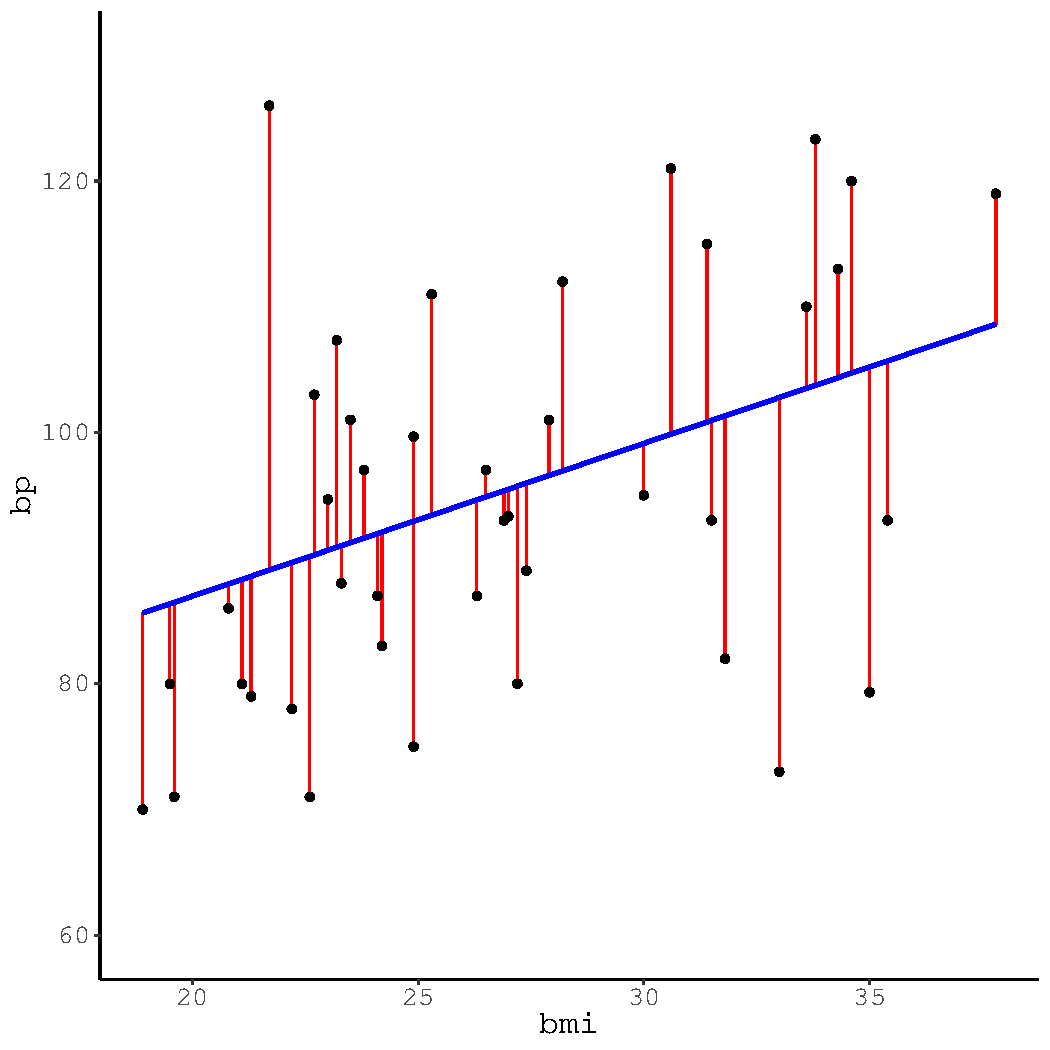
\includegraphics[width=\maxwidth]{figure/unnamed-chunk-4-1} 

}



\end{knitrout}
}
\only<2>{
\begin{knitrout}\footnotesize
\definecolor{shadecolor}{rgb}{0.878, 0.918, 0.933}\color{fgcolor}

{\centering 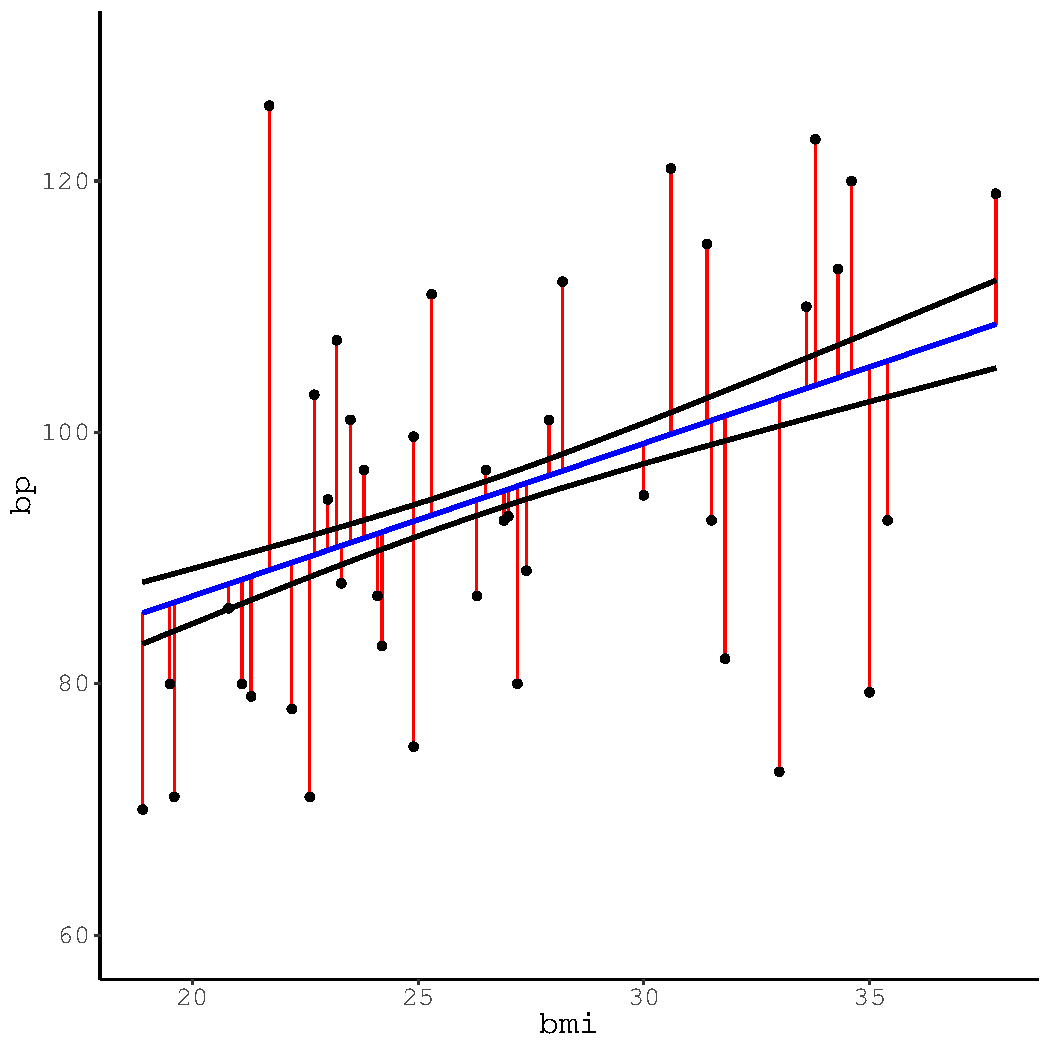
\includegraphics[width=\maxwidth]{figure/unnamed-chunk-5-1} 

}



\end{knitrout}
}
\only<3>{
\begin{knitrout}\footnotesize
\definecolor{shadecolor}{rgb}{0.878, 0.918, 0.933}\color{fgcolor}

{\centering 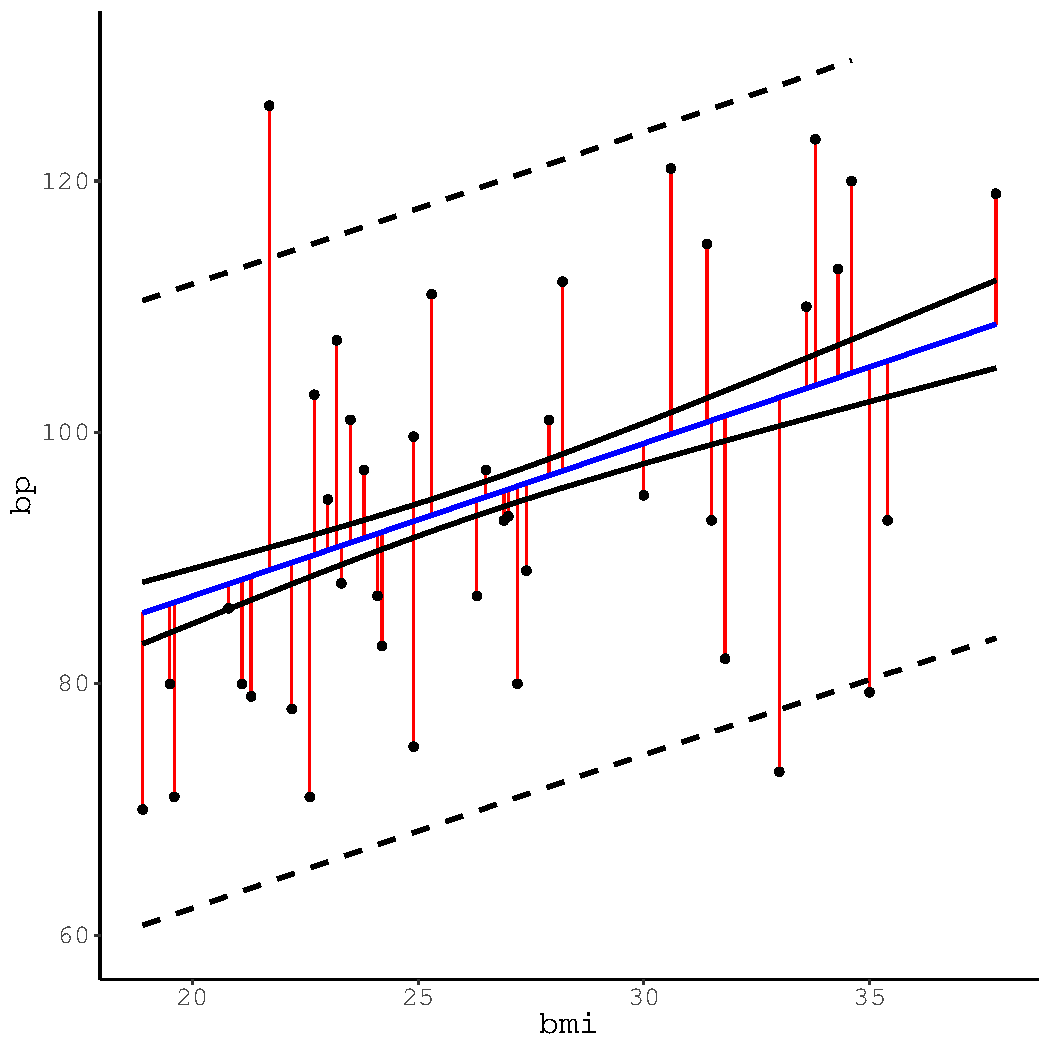
\includegraphics[width=\maxwidth]{figure/unnamed-chunk-6-1} 

}



\end{knitrout}
}

\end{column}
\end{columns}

\end{frame}

\watermarkon %-----------------------------------------------------------------%
 
\begin{frame}{Confidence vs. Prediction Intervals}
  
  Assume we want predictions for a new observation, $X^*$. Then our intervals 
  can be computed as follows:
  \vb
  \begin{itemize}
  \item Confidence interval:
    \begin{align*}
      CI = \hat{Y} \pm t_{crit} \sqrt{\frac{\hat{\sigma}^2}{N} + \frac{\left(X^* - \bar{X}\right)^2}{\left(\sum_{n = 1}^N X_n- \bar{X}\right)^2}}
    \end{align*}
  \item Prediction interval:
    \begin{align*}
      PI = \hat{Y} \pm t_{crit} \sqrt{{\color{red}\hat{\sigma}^2} + \frac{\hat{\sigma}^2}{N} + \frac{\left(X^* - \bar{X}\right)^2}{\left(\sum_{n = 1}^N X_n- \bar{X}\right)^2}}
    \end{align*}
  \end{itemize}
  
\end{frame}

%------------------------------------------------------------------------------%

\begin{frame}{Interval Estimates Example}
  
  Going back to our hypothetical ``new'' patient, we get the following $95\%$ 
  interval estimates:
  \begin{align*}
    95\% CI_{\hat{Y}_{LDL}} &= [115.599; 129.327]\\[8pt]
    95\% PI &= [66.559; 178.368]
  \end{align*}
  \vx{-12}
  \begin{itemize}
  \item We can be 95\% confident that the \underline{average \emph{LDL}} of 
    patients with $BP = 121$, $gluc = 89$, and $BMI = 30.6$
    will be somewhere between 115.599 and 129.327.
    \vb
  \item We can be 95\% confident that the \underline{\emph{LDL} of a specific 
    patient} with $BP = 121$, $gluc = 89$, and $BMI = 30.6$
    will be somewhere between 66.559 and 178.368.
  \end{itemize}
  
\end{frame}

%------------------------------------------------------------------------------%

\begin{frame}{Specifying Predictive Models}
  
  When focused on inferences about regression coefficients, we care very much
  about the predictors entered into the model.  
  \vb
  \begin{itemize}
  \item Partial regression coefficients must be interpreted as controlling for
    all other predictors. 
  \end{itemize}
  \vb
  \pause
  When focused on prediction, we often don't care as much about the
  specific variables that enter the model.  
  \vb
  \begin{itemize}
  \item We prefer whatever set of features produces the best predictive
    performance.  
    \vb
  \item We may want to know which are the ``best'' predictors.
    \vc
    \begin{itemize}
    \item We usually want the data to ``give'' us this answer.
    \end{itemize}
  \end{itemize}
  
\end{frame}

\watermarkoff %----------------------------------------------------------------%

\begin{frame}{\textsc{Aside}: Polynomial Regression}
  
  \begin{columns}
    \begin{column}{0.5\textwidth}
      
      We may hypothesize a curvilinear relationship between $X$ and $Y$.
      \vc
      \begin{itemize}
      \item Polynomial regression adds powered transformations of the
        predictors into the model.
        \vc
      \item Polynomial terms (i.e., power terms) model curvature in the
        relationships.
      \end{itemize}
      
    \end{column}
    \begin{column}{0.5\textwidth}
      
\begin{knitrout}\footnotesize
\definecolor{shadecolor}{rgb}{0.878, 0.918, 0.933}\color{fgcolor}

{\centering 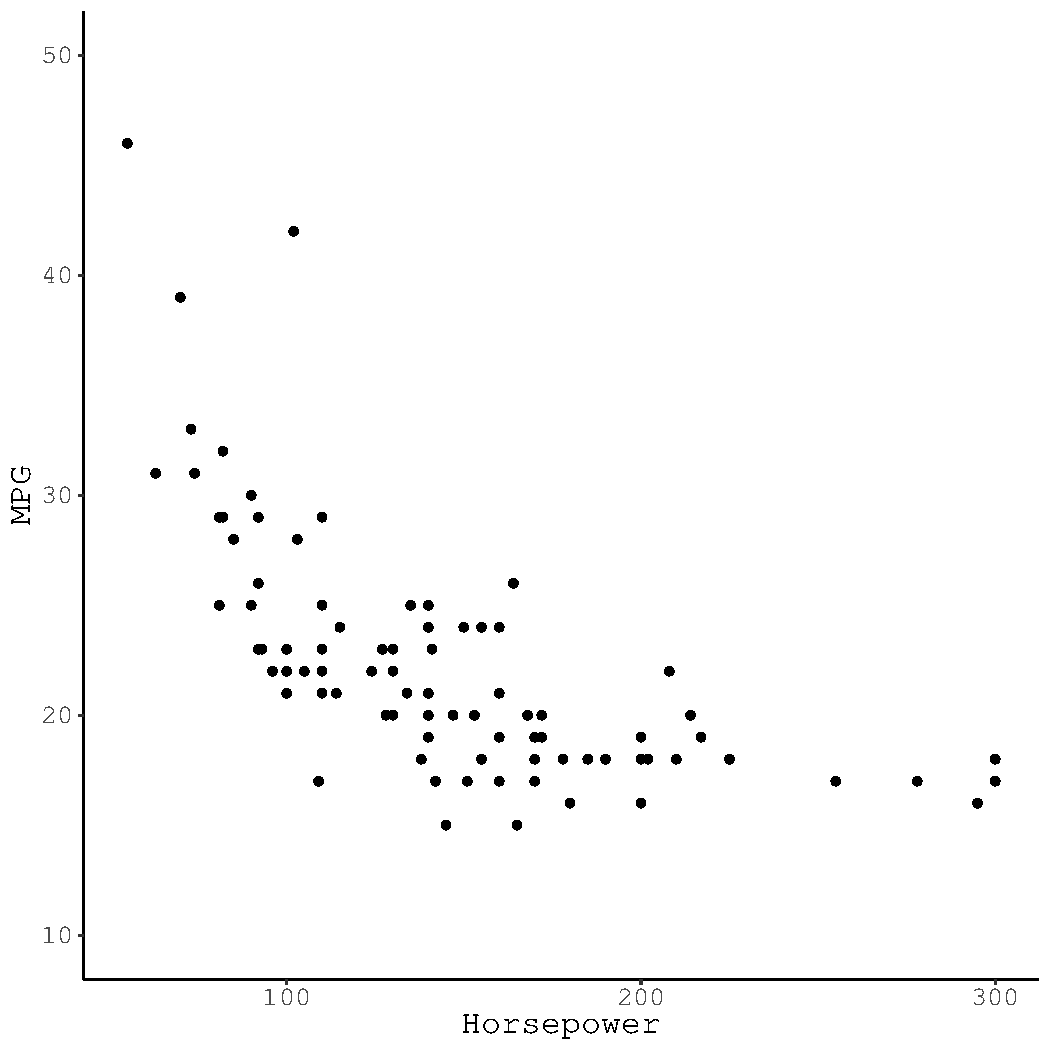
\includegraphics[width=\maxwidth]{figure/unnamed-chunk-7-1} 

}



\end{knitrout}

\end{column}
\end{columns}

\end{frame}

%------------------------------------------------------------------------------%

\begin{frame}{\textsc{Aside}: Polynomial Regression}
  
  \begin{columns}
    \begin{column}{0.5\textwidth}
      Polynomials are one way to model curvilinear relationships.
      \vb
      \begin{itemize}  
      \item {\color{blue}$\hat{Y}_{mpg} = \hat{\beta}_0 + \hat{\beta}_1 X_{hp}$}
        \vb
      \item {\color{red}$\hat{Y}_{mpg} = \hat{\beta}_0 + \hat{\beta}_1 X_{hp} + 
        \hat{\beta}_2 X_{hp}^2$}
        \vb
      \item {\color{violet}$\hat{Y}_{mpg} = \hat{\beta}_0 + \hat{\beta}_1 X_{hp} + 
        \hat{\beta}_2 X_{hp}^2 + \hat{\beta}_3 X_{hp}^3$}
      \end{itemize}
    \end{column}
    
    \begin{column}{0.5\textwidth}
      
\begin{knitrout}\footnotesize
\definecolor{shadecolor}{rgb}{0.878, 0.918, 0.933}\color{fgcolor}

{\centering 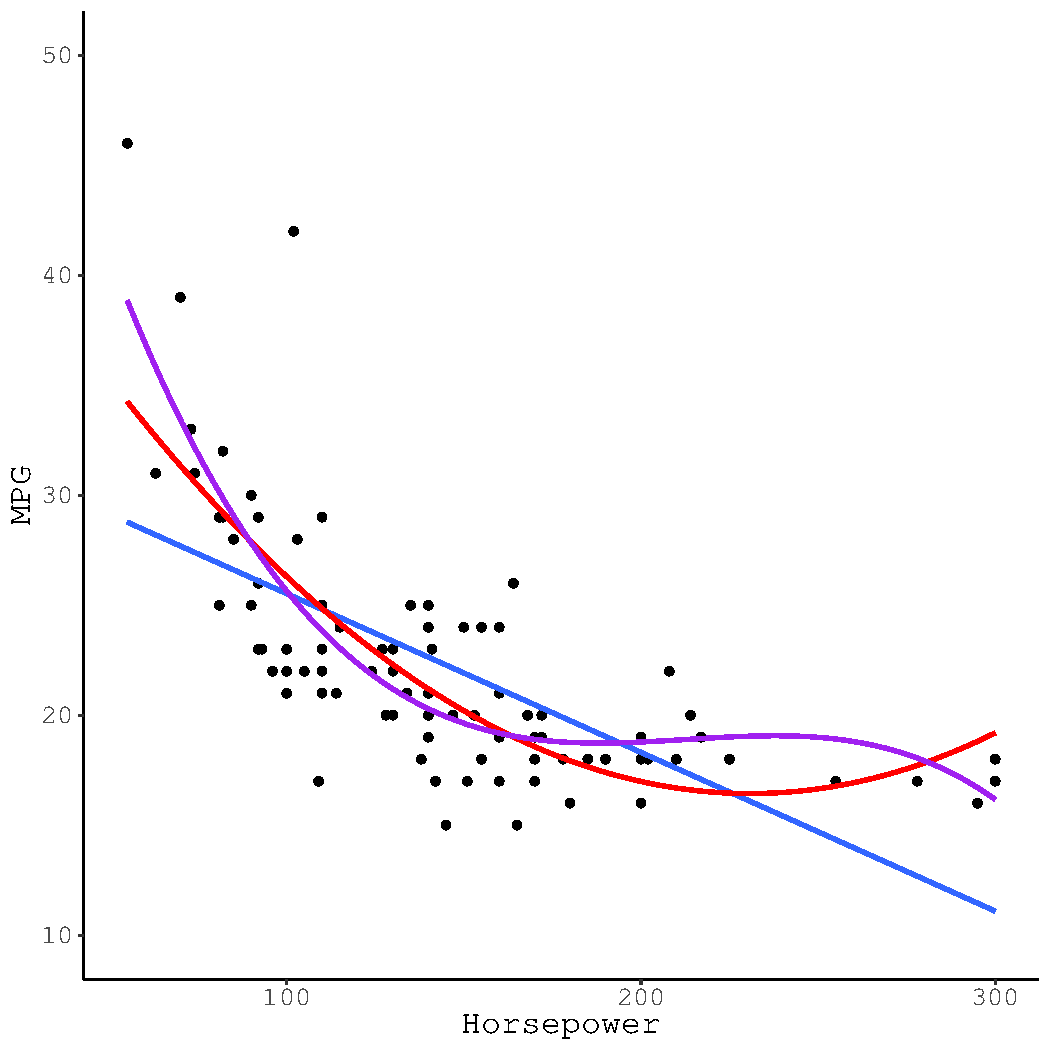
\includegraphics[width=\maxwidth]{figure/unnamed-chunk-8-1} 

}



\end{knitrout}

\end{column}
\end{columns}

\end{frame}

%------------------------------------------------------------------------------%

\begin{frame}{Evaluating Predictive Performance}
  
  \begin{columns}
    \begin{column}{0.5\textwidth}
      
      How do we assess ``good'' prediction?
      \vb
      \begin{itemize}
      \item Can we simply find the model that best predicts the data used to
        train the model?  
        \vb
      \item What are we trying to do when building a predictive model?  
        \vb
      \item Can we quantify this objective with some type of fit measure?
      \end{itemize}
  
      \end{column}
    
    \begin{column}{0.5\textwidth}
      
\begin{knitrout}\footnotesize
\definecolor{shadecolor}{rgb}{0.878, 0.918, 0.933}\color{fgcolor}

{\centering 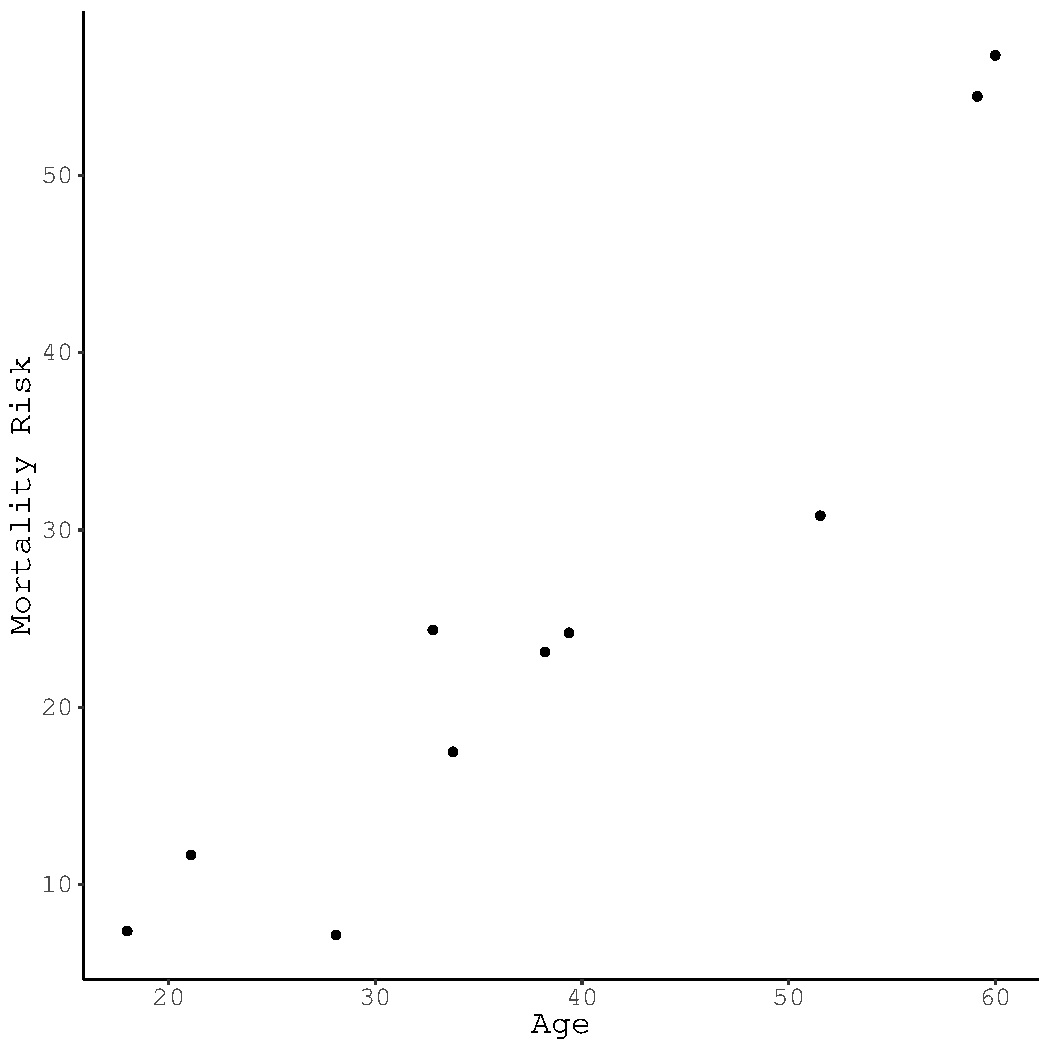
\includegraphics[width=\maxwidth]{figure/unnamed-chunk-9-1} 

}



\end{knitrout}

\end{column}
\end{columns}

\end{frame}

%------------------------------------------------------------------------------%

\begin{frame}{Different Possible Models}
  
  \begin{columns}
    \begin{column}{0.5\textwidth}
        
\begin{knitrout}\footnotesize
\definecolor{shadecolor}{rgb}{0.878, 0.918, 0.933}\color{fgcolor}

{\centering 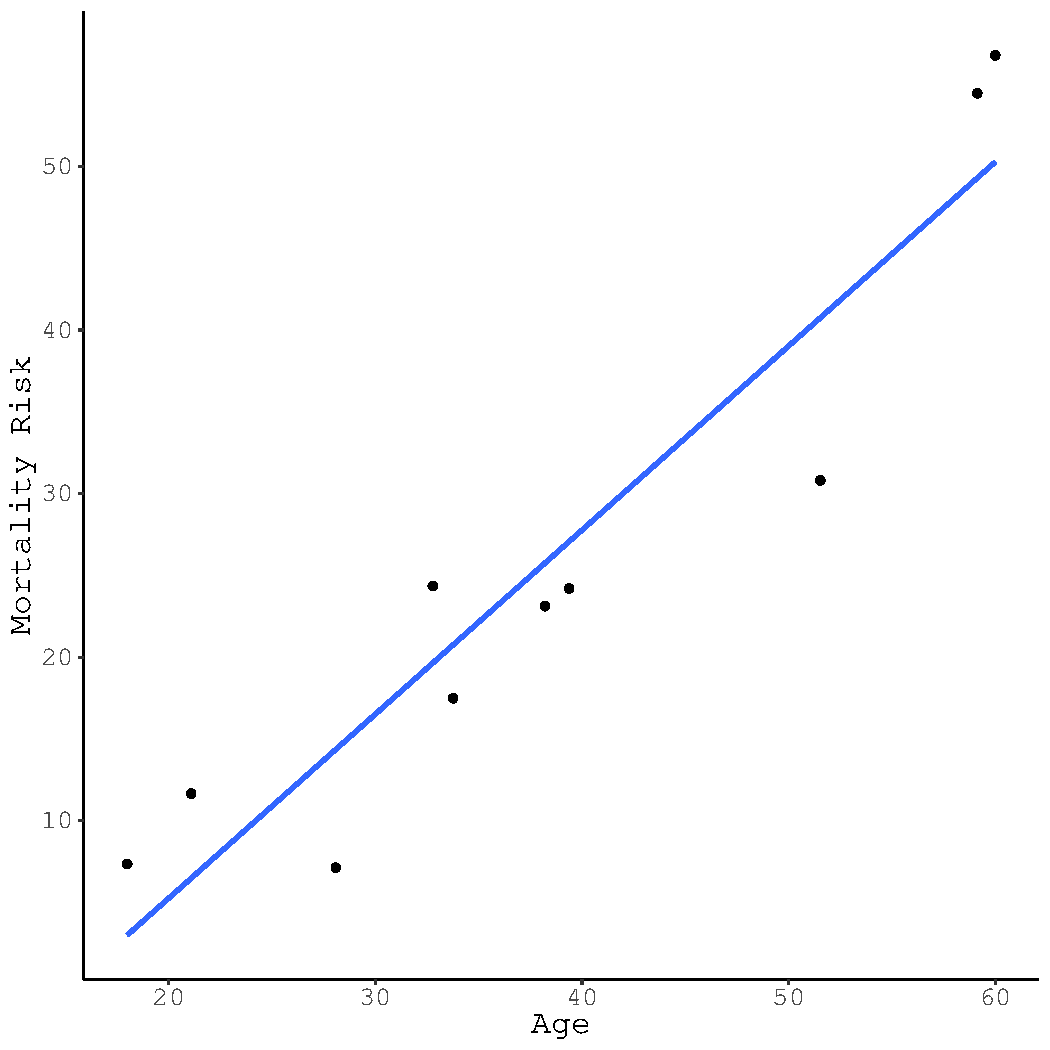
\includegraphics[width=0.6\textwidth]{figure/unnamed-chunk-10-1} 

}



\end{knitrout}

\end{column}

\begin{column}{0.5\textwidth}
  
\begin{knitrout}\footnotesize
\definecolor{shadecolor}{rgb}{0.878, 0.918, 0.933}\color{fgcolor}

{\centering 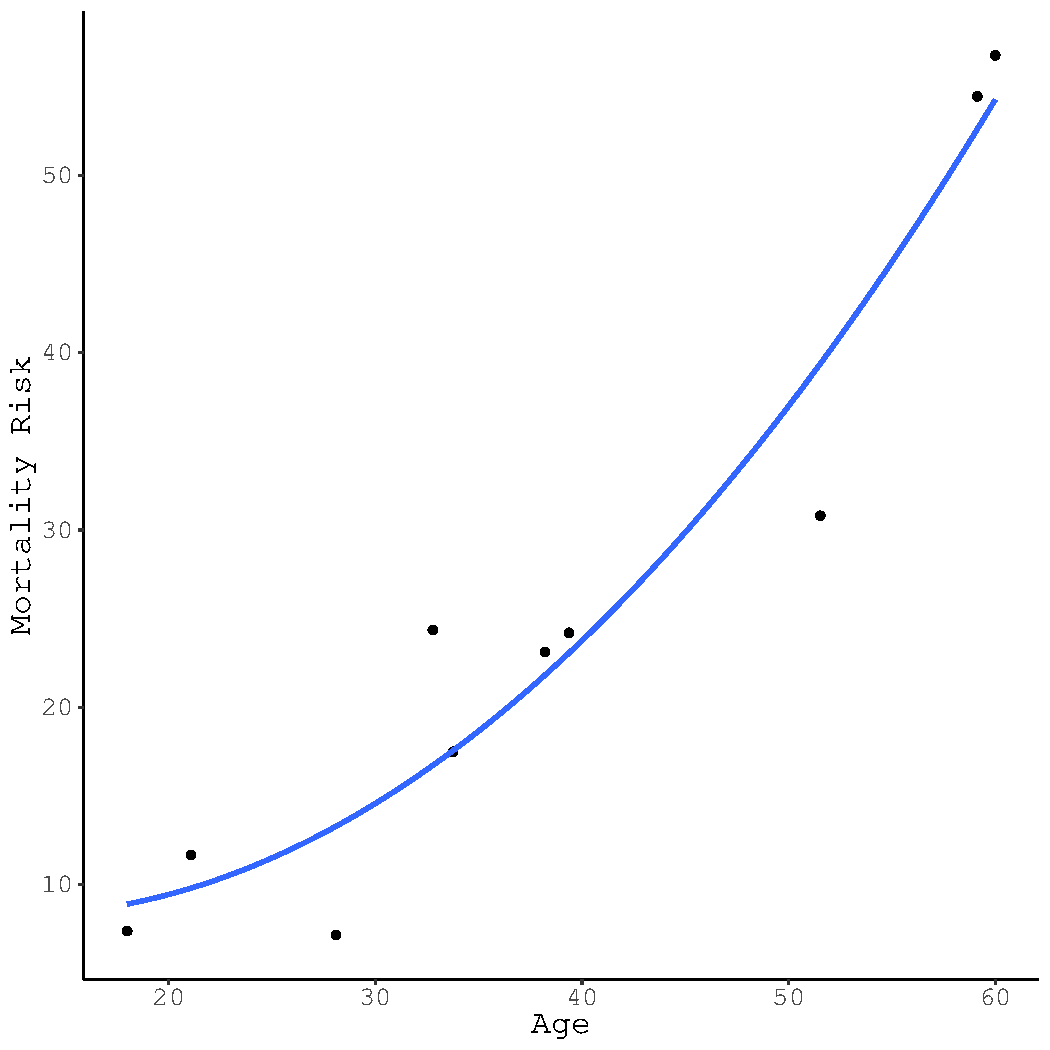
\includegraphics[width=0.6\textwidth]{figure/unnamed-chunk-11-1} 

}



\end{knitrout}

\end{column}
\end{columns}

  \va
  
\begin{columns}
  \begin{column}{0.5\textwidth}
    
\begin{knitrout}\footnotesize
\definecolor{shadecolor}{rgb}{0.878, 0.918, 0.933}\color{fgcolor}

{\centering 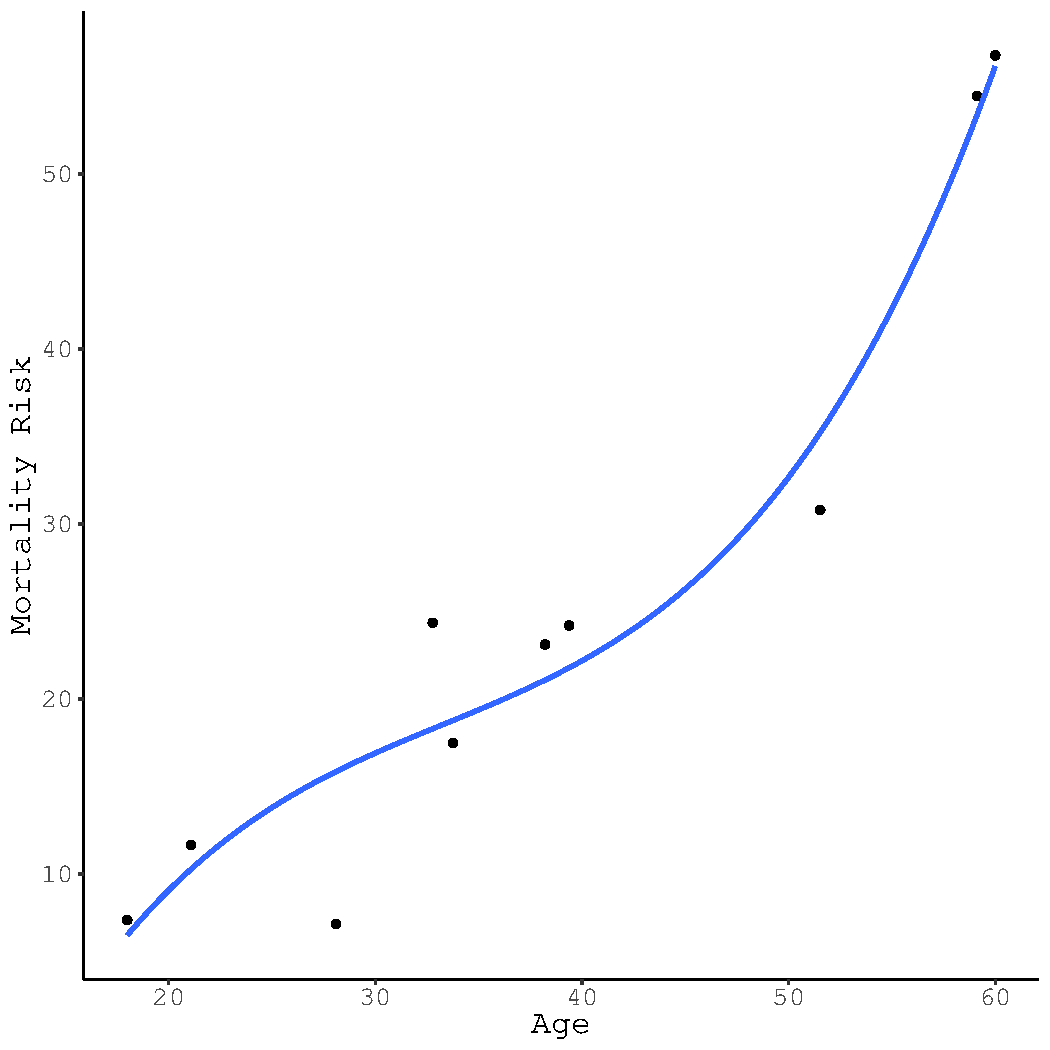
\includegraphics[width=0.6\textwidth]{figure/unnamed-chunk-12-1} 

}



\end{knitrout}

\end{column}
  
\begin{column}{0.5\textwidth}
  
\begin{knitrout}\footnotesize
\definecolor{shadecolor}{rgb}{0.878, 0.918, 0.933}\color{fgcolor}

{\centering 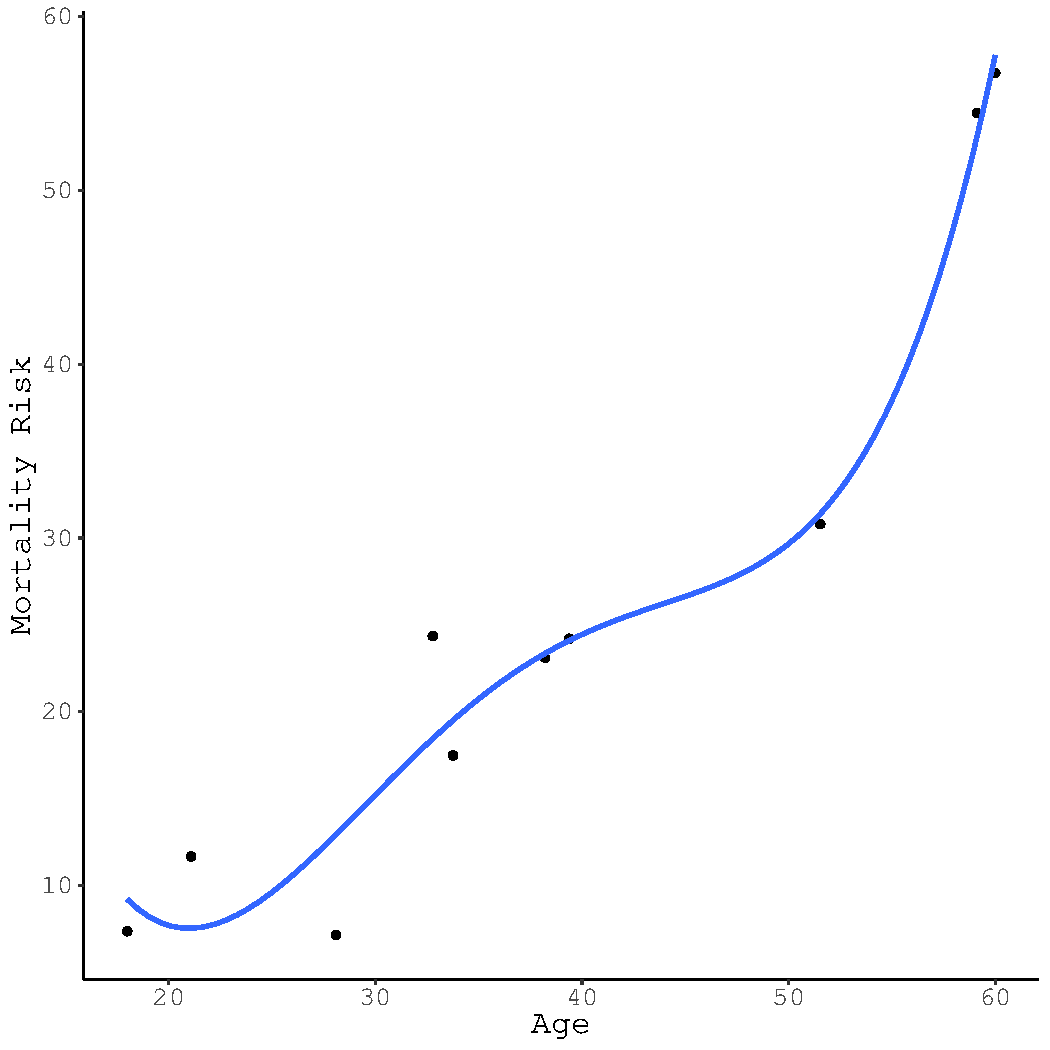
\includegraphics[width=0.6\textwidth]{figure/unnamed-chunk-13-1} 

}



\end{knitrout}

\end{column}
\end{columns}

\end{frame} 
  
%------------------------------------------------------------------------------%

\begin{frame}{Over-fitting}
  
  \begin{columns}
    \begin{column}{0.5\textwidth}
      
      We can easily go too far.
      \vb
      \begin{itemize}
      \item Enough polynomial terms will exactly replicate any data.  
        \vb
      \item Is this what we're trying to do?  
        \vb
      \item What kind of issues arise in the extreme case?
      \end{itemize}
      
    \end{column}
    
    \begin{column}{0.5\textwidth}
      
\begin{knitrout}\footnotesize
\definecolor{shadecolor}{rgb}{0.878, 0.918, 0.933}\color{fgcolor}

{\centering 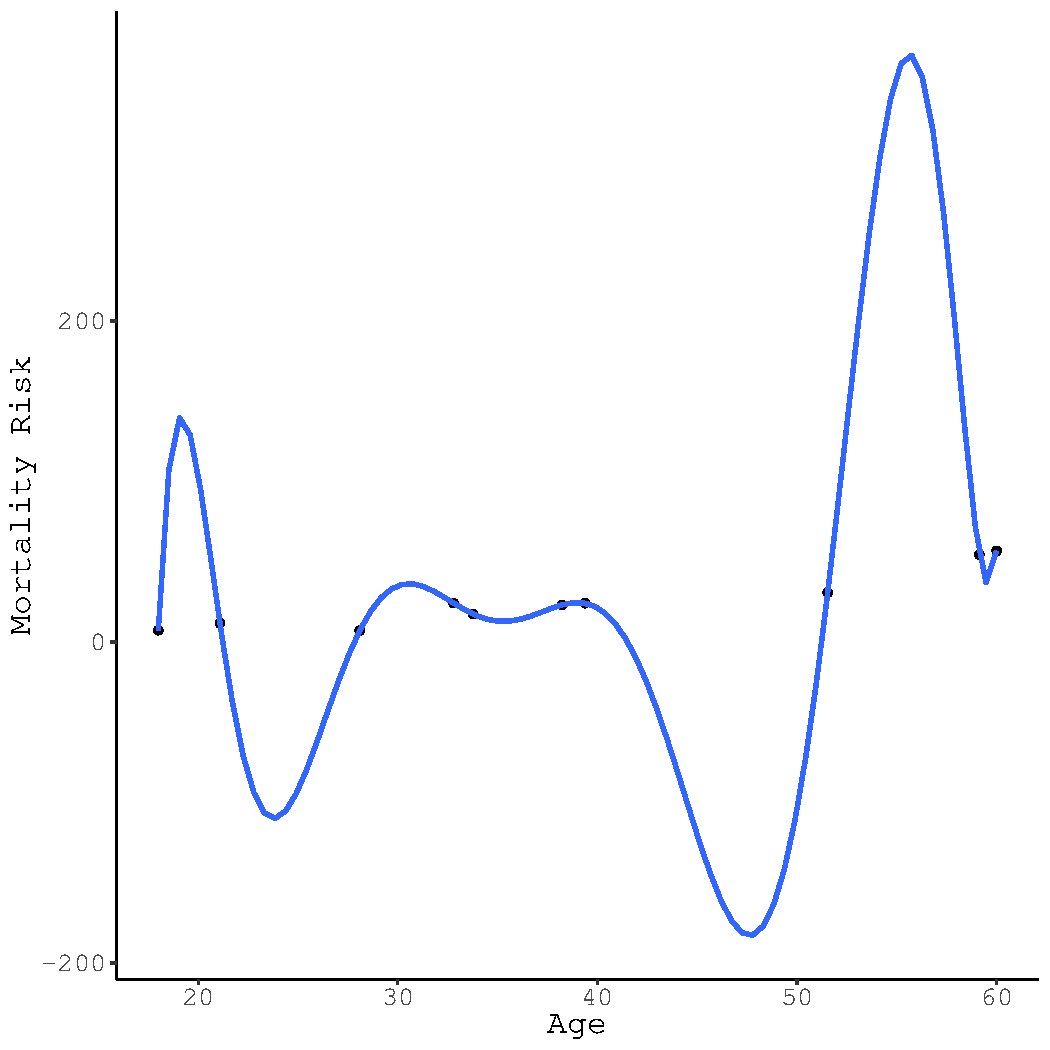
\includegraphics[width=\maxwidth]{figure/unnamed-chunk-14-1} 

}



\end{knitrout}

\end{column}
\end{columns}

\end{frame}

%------------------------------------------------------------------------------%

\begin{frame}{Consequences of Over-fitting}
  
  \begin{columns}
    \begin{column}{0.5\textwidth}
      
      Should we be pleased to be able to perfectly predict mortality risk? 
      \vb
      \begin{itemize}
      \item Is our model useful?
        \vc
      \item What happens if we try to apply our fitted model to new data?
      \end{itemize}
      
    \end{column}
    
    \pause
    
    \begin{column}{0.5\textwidth}
      
\begin{knitrout}\footnotesize
\definecolor{shadecolor}{rgb}{0.878, 0.918, 0.933}\color{fgcolor}

{\centering 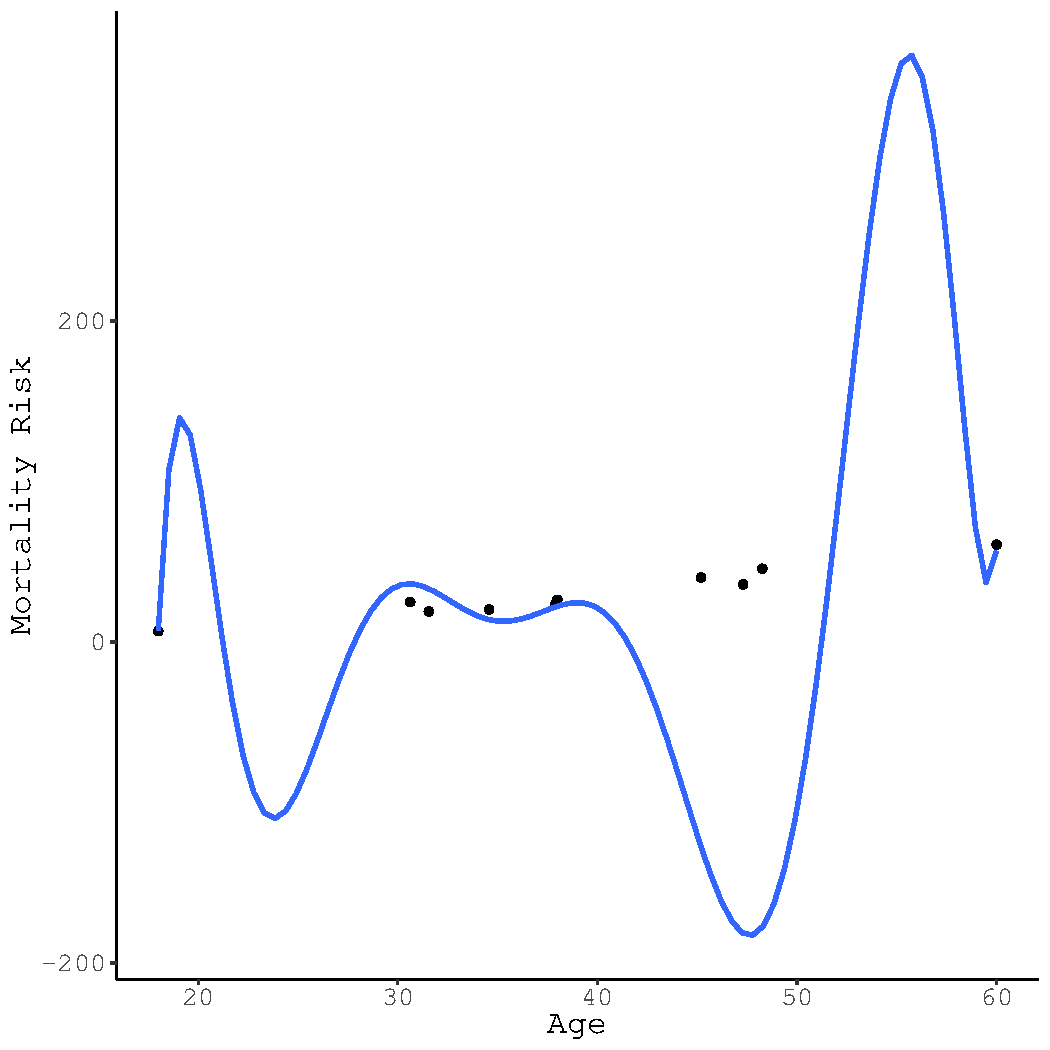
\includegraphics[width=\maxwidth]{figure/unnamed-chunk-15-1} 

}



\end{knitrout}

\end{column}
\end{columns}

\end{frame}

%------------------------------------------------------------------------------%

\begin{frame}{Correct Fit}
  
  Let's try something a bit more reasonable.\\
  \vb
  \begin{columns}
    \begin{column}{0.5\textwidth}
      
\begin{knitrout}\footnotesize
\definecolor{shadecolor}{rgb}{0.878, 0.918, 0.933}\color{fgcolor}

{\centering 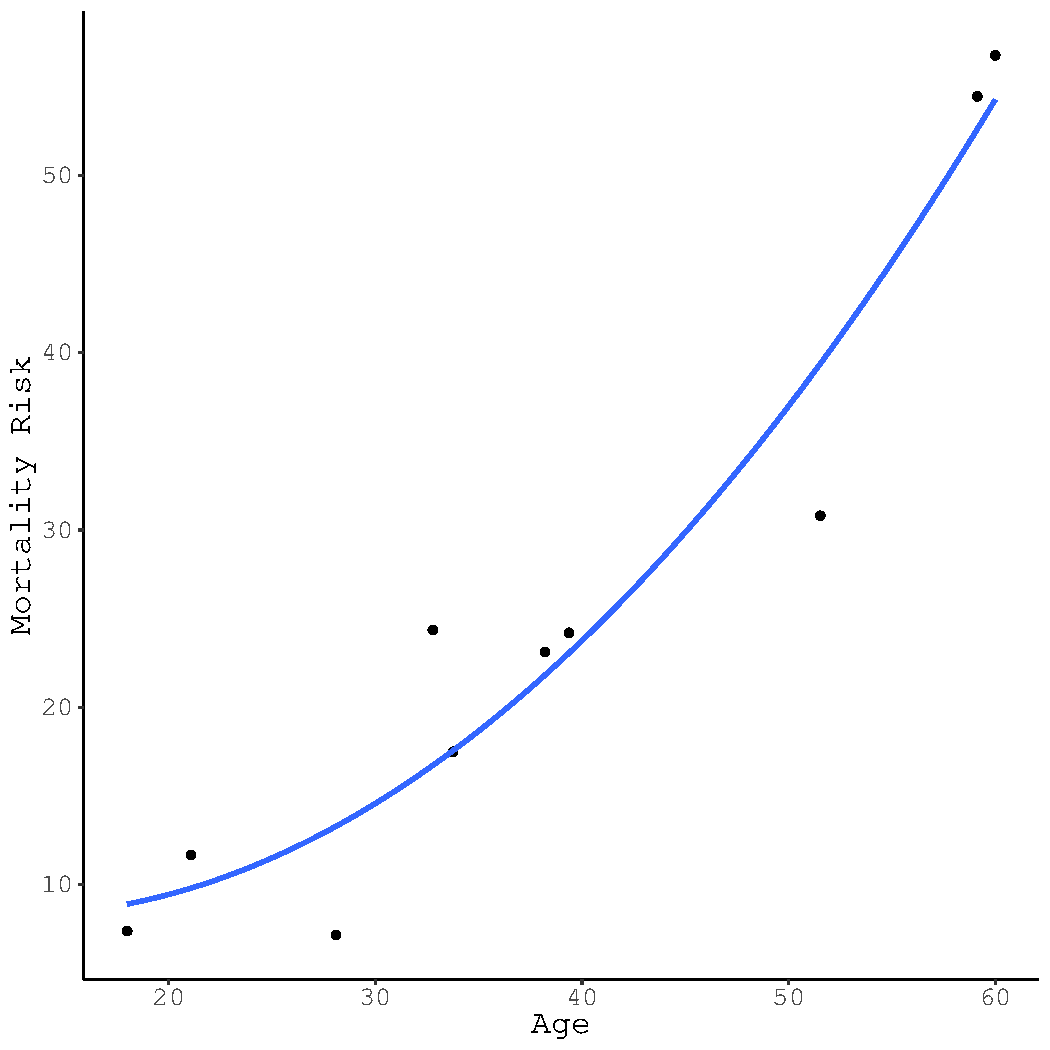
\includegraphics[width=\maxwidth]{figure/unnamed-chunk-16-1} 

}



\end{knitrout}

\end{column}

\begin{column}{0.5\textwidth}
  
\begin{knitrout}\footnotesize
\definecolor{shadecolor}{rgb}{0.878, 0.918, 0.933}\color{fgcolor}

{\centering 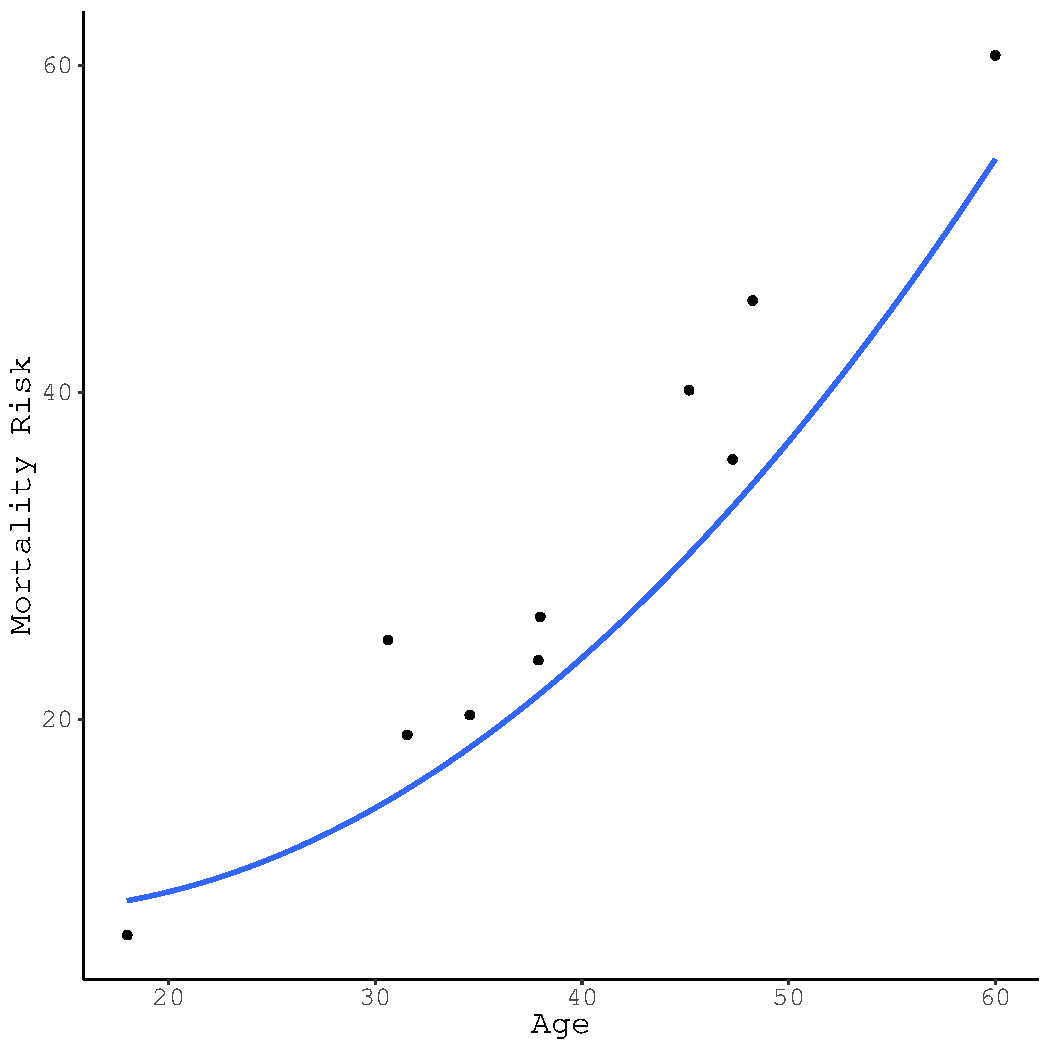
\includegraphics[width=\maxwidth]{figure/unnamed-chunk-17-1} 

}



\end{knitrout}

\end{column}
\end{columns}

\end{frame}

\watermarkon %-----------------------------------------------------------------%

\begin{frame}{A Sensible Goal}
  
  Our goal is to train a model that can best predict \emph{new data}.
  \vc
  \begin{itemize}
  \item The predictive performance on the training data is immaterial.
  \item We can always fit the training data arbitrarily well.
  \item Fit to the training data will always be at-odds with fit to future data.
  \end{itemize}
  \vc
  This conflict is the driving force behind the \emph{bias-variance trade-off}

\end{frame}

%------------------------------------------------------------------------------%

\begin{frame}{Model Fit for Prediction}
  
  When assessing predictive performance, we will most often use the \emph{mean
    squared error} (MSE) as our criterion.
  \vb
  \begin{align*}
    MSE &= \frac{1}{N} \sum_{n = 1}^N \left(Y_n - \hat{Y}_n\right)^2\\
    &= \frac{1}{N} \sum_{n = 1}^N \left(Y_n - \hat{\beta}_0 - 
    \sum_{p = 1}^P \hat{\beta}_p X_{np} \right)^2\\
    &= \frac{RSS}{N}
  \end{align*}
  
\end{frame}

%------------------------------------------------------------------------------%

\begin{frame}{Training vs. Test MSE}
  
  The MSE on the preceding slide (i.e., the only MSE we've considered, so far) 
  is computing entirely from training data.
  \vb
  \begin{itemize}
  \item \emph{Training MSE}
  \end{itemize}
  \vb
  What we want is a measure of fit to new, \emph{testing} data.
  \vb
  \begin{itemize}
  \item \emph{Test MSE}
    \vb
  \item Given $M$ new observations $\{Y_m, X_{m1}, X_{m2}, \ldots, X_{mP}\}$, 
    and a fitted regression model, $f(\mathbf{X})$, defined by the 
    coefficients $\{\hat{\beta}_0, \hat{\beta}_1, \hat{\beta}_2, \ldots, 
    \hat{\beta}_P\}$, the \emph{Test MSE} is given by:
    \begin{align*}
      MSE &= \frac{1}{M} \sum_{m = 1}^M \left(Y_m - \hat{\beta}_0 - 
      \sum_{p = 1}^P \hat{\beta}_p X_{mp} \right)^2\\
    \end{align*}
  \end{itemize}
  
\end{frame}

\watermarkoff %----------------------------------------------------------------%

\begin{frame}{Training vs. Test MSE}
  
  \begin{columns}
    \begin{column}{0.5\textwidth}
      
      \textcolor{red}{Training MSE} will always decrease in response to 
      increased model complexity.  
      \vb
      \begin{itemize}
      \item Note the red line in the plot.
      \end{itemize}
      \vb
      \textcolor{blue}{Test MSE} will reach a minimum at some ``optimal'' level 
      of model complexity.
      \vb
      \begin{itemize}
      \item Further complicating the model will increase Test MSE.
        \vb
      \item Note the blue line.
      \end{itemize}
      
    \end{column}
    
    \begin{column}{0.5\textwidth}
      
\begin{knitrout}\footnotesize
\definecolor{shadecolor}{rgb}{0.878, 0.918, 0.933}\color{fgcolor}

{\centering 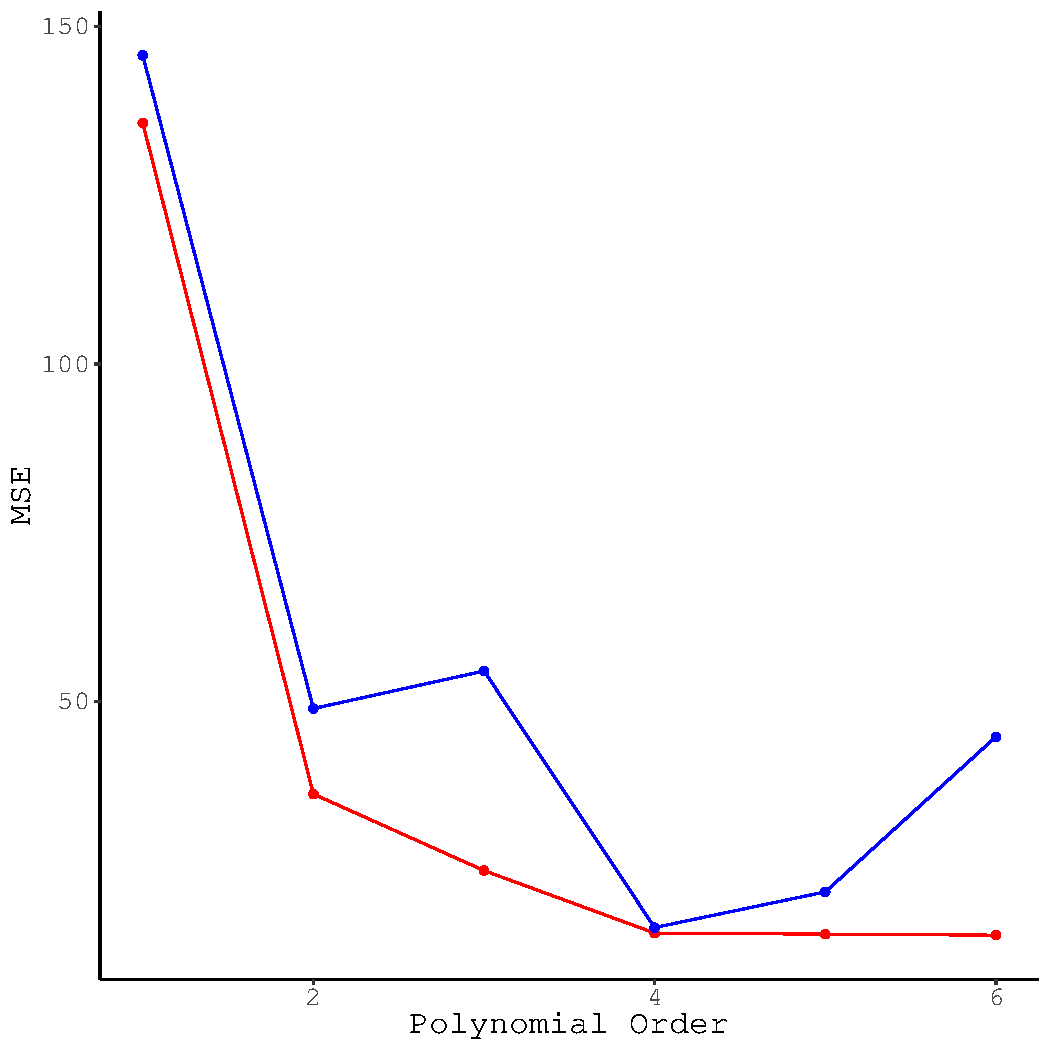
\includegraphics[width=\maxwidth]{figure/mse_fig-1} 

}



\end{knitrout}

\end{column}
\end{columns}

\end{frame}

\watermarkon %-----------------------------------------------------------------%

\begin{frame}{Training vs. Test MSE}

  In the last lecture, we compared the following models:
  \begin{align}
    Y_{BP} &= \beta_0 + \beta_1 X_{age} + \beta_2 X_{LDL} + \beta_3 X_{HDL} + 
    \beta_4 X_{BMI} + \varepsilon \label{fullMod}\\
    Y_{BP} &= \beta_0 + \beta_1 X_{age} + \beta_2 X_{BMI} + 
    \varepsilon \label{resMod}
  \end{align}
  \vx{-12}
  \begin{itemize}
  \item The $\Delta R^2$ test suggested that the loss in fit between Model 
    \ref{fullMod} and Model \ref{resMod} was trivial.
    \vc
  \item The Training MSE values suggested that Model \ref{fullMod} should be 
    preferred.
  \end{itemize}
  \vb
  What happens when we do the comparison based on Test MSE instead of Training 
  MSE?
  
\end{frame}

\watermarkoff %----------------------------------------------------------------%

\begin{frame}[fragile]{Training vs. Test MSE}
  
\begin{knitrout}\footnotesize
\definecolor{shadecolor}{rgb}{0.878, 0.918, 0.933}\color{fgcolor}\begin{kframe}
\begin{alltt}
\hlkwd{set.seed}\hlstd{(}\hlnum{235711}\hlstd{)}

\hlcom{## Read in the data:}
\hlstd{dDat} \hlkwb{<-} \hlkwd{readRDS}\hlstd{(}\hlstr{"../data/diabetes.rds"}\hlstd{)}

\hlcom{## Split data into training and testing sets:}
\hlstd{ind}  \hlkwb{<-} \hlkwd{sample}\hlstd{(}\hlnum{1} \hlopt{:} \hlkwd{nrow}\hlstd{(dDat))}
\hlstd{dat0} \hlkwb{<-} \hlstd{dDat[ind[}\hlnum{1} \hlopt{:} \hlnum{400}\hlstd{], ]}   \hlcom{# Training data}
\hlstd{dat1} \hlkwb{<-} \hlstd{dDat[ind[}\hlnum{401} \hlopt{:} \hlnum{442}\hlstd{], ]} \hlcom{# Testing data}

\hlcom{## Fit the models:}
\hlstd{outF} \hlkwb{<-} \hlkwd{lm}\hlstd{(bp} \hlopt{~} \hlstd{age} \hlopt{+} \hlstd{bmi} \hlopt{+} \hlstd{ldl} \hlopt{+} \hlstd{hdl,} \hlkwc{data} \hlstd{= dat0)}
\hlstd{outR} \hlkwb{<-} \hlkwd{lm}\hlstd{(bp} \hlopt{~} \hlstd{age} \hlopt{+} \hlstd{bmi,} \hlkwc{data} \hlstd{= dat0)}

\hlcom{## Compute training MSEs:}
\hlstd{trainMseF} \hlkwb{<-} \hlkwd{MSE}\hlstd{(}\hlkwc{y_pred} \hlstd{=} \hlkwd{predict}\hlstd{(outF),} \hlkwc{y_true} \hlstd{= dat0}\hlopt{$}\hlstd{bp)}
\hlstd{trainMseR} \hlkwb{<-} \hlkwd{MSE}\hlstd{(}\hlkwc{y_pred} \hlstd{=} \hlkwd{predict}\hlstd{(outR),} \hlkwc{y_true} \hlstd{= dat0}\hlopt{$}\hlstd{bp)}
\end{alltt}
\end{kframe}
\end{knitrout}

\end{frame}

\watermarkon %-----------------------------------------------------------------%

\begin{frame}[fragile]{Training vs. Test MSE}
  
\begin{knitrout}\footnotesize
\definecolor{shadecolor}{rgb}{0.878, 0.918, 0.933}\color{fgcolor}\begin{kframe}
\begin{alltt}
\hlcom{## Compute testing MSEs:}
\hlstd{testMseF} \hlkwb{<-} \hlkwd{MSE}\hlstd{(}\hlkwc{y_pred} \hlstd{=} \hlkwd{predict}\hlstd{(outF,} \hlkwc{newdata} \hlstd{= dat1),}
                \hlkwc{y_true} \hlstd{= dat1}\hlopt{$}\hlstd{bp)}
\hlstd{testMseR} \hlkwb{<-} \hlkwd{MSE}\hlstd{(}\hlkwc{y_pred} \hlstd{=} \hlkwd{predict}\hlstd{(outR,} \hlkwc{newdata} \hlstd{= dat1),}
                \hlkwc{y_true} \hlstd{= dat1}\hlopt{$}\hlstd{bp)}
\end{alltt}
\end{kframe}
\end{knitrout}

Compare the two approaches:

% latex table generated in R 4.0.2 by xtable 1.8-4 package
% Fri Sep 18 13:27:34 2020
\begin{table}[ht]
\centering
\begin{tabular}{rrr}
  \toprule
 & Full & Restricted \\ 
  \midrule
Train & 147.72 & 148.44 \\ 
  Test & 141.25 & 138.02 \\ 
   \bottomrule
\end{tabular}
\caption{MSE Values} 
\end{table}


\end{frame}

%------------------------------------------------------------------------------%

\begin{frame}{Cross Validation}

  To train a model that best predicts new data, we use \emph{cross-validation}
  to choose the best model from a pool of candidates.  
  \vb
  \begin{itemize}
  \item Given a set $\mathcal{F} = \{f_1(\mathbf{X}), f_2(\mathbf{X}), \ldots, 
    f_J(\mathbf{X})\}$ of $J$ competing models, the simplest form of 
    cross-validation entails the following:
    \vb
    \begin{enumerate}
    \item Split the sample into two, disjoint sub-samples:
      \begin{itemize}
      \item \emph{Training} data
      \item \emph{Testing} data
      \end{itemize}
      \vc
    \item Estimate a candidate model, $f_j(\mathbf{X})$, on the training data. 
      \label{train}
      \vb
    \item Check the predictive performance of $\hat{f}_j(\mathbf{X})$ on the 
      testing data. \label{test}
      \vb
    \item Repeat Steps \ref{train} and \ref{test} for all candidate models in 
      $\mathcal{F}$.
      \vb
    \item Pick the $\hat{f}_j(\mathbf{X})$ that best predicts the testing data.
    \end{enumerate}
  \end{itemize}
  
\end{frame}

%------------------------------------------------------------------------------%

\begin{frame}{Estimating Prediction Error}
  
  The split-sample cross-validation scheme described above will underestimate 
  prediction error.
  \vc
  \begin{itemize}
  \item The same testing data are re-used to estimate the relative prediction 
    error of the candidate models.
    \vc
  \item If we need a good estimate of our final model's prediction error, we 
    need to complicate the split-sample procedure slightly:
    \pause
    \vc
    \begin{enumerate}
    \item Split the sample into \emph{three} disjoint subsets:
      \begin{itemize}
      \item \emph{Training} data, \emph{validation} data, and \emph{testing} 
        data
      \end{itemize}
      \vc
    \item Use the training and validation data to choose the best model via the 
      cross-validation procedure described earlier.
      \vc
    \item Fit the chosen model to the combined training and validation data. 
      \label{fitStep}
      \vc
    \item Use the Step \ref{fitStep} model to generate predictions from the 
      testing data.
      \vc
    \item Use the test-set predictions to estimate prediction error.
    \end{enumerate}
  \end{itemize}
  
\end{frame}
  
\watermarkoff %----------------------------------------------------------------%

\begin{frame}[fragile, allowframebreaks]{Estimating Prediction Error}
  
\begin{knitrout}\footnotesize
\definecolor{shadecolor}{rgb}{0.878, 0.918, 0.933}\color{fgcolor}\begin{kframe}
\begin{alltt}
\hlkwd{set.seed}\hlstd{(}\hlnum{235711}\hlstd{)}

\hlcom{## Split data into training, testing, and validation sets:}
\hlstd{ind}  \hlkwb{<-} \hlkwd{sample}\hlstd{(}\hlnum{1} \hlopt{:} \hlkwd{nrow}\hlstd{(dDat))}
\hlstd{dat0} \hlkwb{<-} \hlstd{dDat[ind[}\hlnum{1} \hlopt{:} \hlnum{350}\hlstd{], ]}   \hlcom{# Training data}
\hlstd{dat1} \hlkwb{<-} \hlstd{dDat[ind[}\hlnum{351} \hlopt{:} \hlnum{400}\hlstd{], ]} \hlcom{# Validation data}
\hlstd{dat2} \hlkwb{<-} \hlstd{dDat[ind[}\hlnum{401} \hlopt{:} \hlnum{442}\hlstd{], ]} \hlcom{# Testing data}

\hlcom{## Fit models to training data:}
\hlstd{outF} \hlkwb{<-} \hlkwd{lm}\hlstd{(bp} \hlopt{~} \hlstd{age} \hlopt{+} \hlstd{bmi} \hlopt{+} \hlstd{ldl} \hlopt{+} \hlstd{hdl,} \hlkwc{data} \hlstd{= dat0)}
\hlstd{outR} \hlkwb{<-} \hlkwd{lm}\hlstd{(bp} \hlopt{~} \hlstd{age} \hlopt{+} \hlstd{bmi,} \hlkwc{data} \hlstd{= dat0)}
\end{alltt}
\end{kframe}
\end{knitrout}

\pagebreak

\begin{knitrout}\footnotesize
\definecolor{shadecolor}{rgb}{0.878, 0.918, 0.933}\color{fgcolor}\begin{kframe}
\begin{alltt}
\hlcom{## Compute validation MSEs:}
\hlstd{validMseF} \hlkwb{<-} \hlkwd{MSE}\hlstd{(}\hlkwc{y_pred} \hlstd{=} \hlkwd{predict}\hlstd{(outF,} \hlkwc{newdata} \hlstd{= dat1),}
                 \hlkwc{y_true} \hlstd{= dat1}\hlopt{$}\hlstd{bp)}
\hlstd{validMseR} \hlkwb{<-} \hlkwd{MSE}\hlstd{(}\hlkwc{y_pred} \hlstd{=} \hlkwd{predict}\hlstd{(outR,} \hlkwc{newdata} \hlstd{= dat1),}
                 \hlkwc{y_true} \hlstd{= dat1}\hlopt{$}\hlstd{bp)}

\hlcom{## Use validation MSEs to choose the best model:}
\hlstd{validMseF}
\end{alltt}
\begin{verbatim}
## [1] 163.6176
\end{verbatim}
\begin{alltt}
\hlstd{validMseR}
\end{alltt}
\begin{verbatim}
## [1] 166.3149
\end{verbatim}
\end{kframe}
\end{knitrout}

\pagebreak



\begin{knitrout}\footnotesize
\definecolor{shadecolor}{rgb}{0.878, 0.918, 0.933}\color{fgcolor}\begin{kframe}
\begin{alltt}
\hlcom{## Pool training and validation data:}
\hlstd{dat01} \hlkwb{<-} \hlkwd{rbind}\hlstd{(dat0, dat1)}
\end{alltt}
\end{kframe}
\end{knitrout}

\begin{knitrout}\footnotesize
\definecolor{shadecolor}{rgb}{0.878, 0.918, 0.933}\color{fgcolor}\begin{kframe}
\begin{alltt}
\hlcom{## Estimate the chosen model:}
\hlstd{outC} \hlkwb{<-} \hlkwd{lm}\hlstd{(bp} \hlopt{~} \hlstd{age} \hlopt{+} \hlstd{bmi} \hlopt{+} \hlstd{ldl} \hlopt{+} \hlstd{hdl,} \hlkwc{data} \hlstd{= dat01)}
\end{alltt}
\end{kframe}
\end{knitrout}



\begin{knitrout}\footnotesize
\definecolor{shadecolor}{rgb}{0.878, 0.918, 0.933}\color{fgcolor}\begin{kframe}
\begin{alltt}
\hlcom{## Estimate prediction error using the testing data:}
\hlstd{predErr} \hlkwb{<-} \hlkwd{MSE}\hlstd{(}\hlkwc{y_pred} \hlstd{=} \hlkwd{predict}\hlstd{(outC,} \hlkwc{newdata} \hlstd{= dat2),}
               \hlkwc{y_true} \hlstd{= dat2}\hlopt{$}\hlstd{bp)}

\hlcom{## This value can be reported as our best estimate of the }
\hlcom{## prediction error:}
\hlstd{predErr}
\end{alltt}
\begin{verbatim}
## [1] 141.2545
\end{verbatim}
\end{kframe}
\end{knitrout}

\end{frame}

\watermarkon %-----------------------------------------------------------------%

\begin{frame}{Different Flavors of Cross-Validation}
  
  In practice, the split-sample cross-validation procedure describe above can be 
  highly variable.
  \vc
  \begin{itemize}
  \item The solution is highly sensitive to the way the sample is split because 
    each model is only training once.
  \end{itemize}
  \vb 
  Split-sample cross-validation can also be wasteful.
  \vc
  \begin{itemize}
  \item We don't need to set aside an entire chunk of data for validation.
  \end{itemize}
  \vb 
  In most cases, we will want to employ a slightly more complex flavor of
  cross-validation: 
  \vc
  \begin{itemize}
  \item \emph{K-fold cross-validation}
  \end{itemize}
  
\end{frame}

%------------------------------------------------------------------------------%

\begin{frame}{\emph{K}-Fold Cross-Validation}
  
  \begin{enumerate}
  \item If you need to estimate prediction error, set aside a testing set.
    \vb
  \item Partition the (remaining) data into $K$ disjoint subsets $C_k = C_1, C_2, 
    \ldots, C_K$.  
    \vb
  \item Conduct $K$ training replications. 
    \vb
    \begin{itemize}
    \item For each training replication, collapse $K - 1$ partitions into 
      a set of training data. 
      \vb
    \item Compute the validation MSE for the $k$th partition, $MSE_k$, by using
      subset $C_k$ as the validation data for the $k$th fitted model.
    \end{itemize}
    \vb
  \item Compute the overall \kfold~error as:
  \end{enumerate}
  \begin{align*}
    CVE = \sum_{k = 1}^K \frac{N_k}{N}MSE_k,
  \end{align*}
  
\end{frame}

\watermarkoff %----------------------------------------------------------------%

\begin{frame}[fragile]{$K$-Fold Cross-Validation}

\begin{knitrout}\footnotesize
\definecolor{shadecolor}{rgb}{0.878, 0.918, 0.933}\color{fgcolor}\begin{kframe}
\begin{alltt}
\hlstd{getCve} \hlkwb{<-} \hlkwa{function}\hlstd{(}\hlkwc{model}\hlstd{,} \hlkwc{data}\hlstd{,} \hlkwc{K}\hlstd{,} \hlkwc{part}\hlstd{) \{}
    \hlcom{## Loop over K repetitions:}
    \hlstd{mse} \hlkwb{<-} \hlkwd{c}\hlstd{()}
    \hlkwa{for}\hlstd{(k} \hlkwa{in} \hlnum{1} \hlopt{:} \hlstd{K) \{}
        \hlcom{## Partition data:}
        \hlstd{train} \hlkwb{<-} \hlstd{data[part} \hlopt{!=} \hlstd{k, ]}
        \hlstd{valid} \hlkwb{<-} \hlstd{data[part} \hlopt{==} \hlstd{k, ]}

        \hlcom{## Fit model, generate predictions, and save MSE:}
        \hlstd{fit}    \hlkwb{<-} \hlkwd{lm}\hlstd{(model,} \hlkwc{data} \hlstd{= train)}
        \hlstd{pred}   \hlkwb{<-} \hlkwd{predict}\hlstd{(fit,} \hlkwc{newdata} \hlstd{= valid)}
        \hlstd{mse[k]} \hlkwb{<-} \hlkwd{MSE}\hlstd{(}\hlkwc{y_pred} \hlstd{= pred,}
                      \hlkwc{y_true} \hlstd{= valid[ ,} \hlkwd{dvName}\hlstd{(fit)])}
    \hlstd{\}}
    \hlcom{## Return the CVE:}
    \hlkwd{mean}\hlstd{(mse)}
\hlstd{\}}
\end{alltt}
\end{kframe}
\end{knitrout}

\end{frame}

%------------------------------------------------------------------------------%

\begin{frame}[fragile]{$K$-Fold Cross-Validation}

\begin{knitrout}\footnotesize
\definecolor{shadecolor}{rgb}{0.878, 0.918, 0.933}\color{fgcolor}\begin{kframe}
\begin{alltt}
\hlcom{## Do K-Fold Cross-Validation with lm():}
\hlstd{cv.lm} \hlkwb{<-} \hlkwa{function}\hlstd{(}\hlkwc{data}\hlstd{,} \hlkwc{models}\hlstd{,} \hlkwc{K}\hlstd{) \{}
    \hlcom{## Create a partition vector:}
    \hlstd{part} \hlkwb{<-} \hlkwd{rep}\hlstd{(}\hlnum{1} \hlopt{:} \hlstd{K,} \hlkwd{nrow}\hlstd{(data)} \hlopt{/} \hlstd{K)}

    \hlcom{## Permute the partition vector:}
    \hlstd{part} \hlkwb{<-} \hlkwd{sample}\hlstd{(part)}

    \hlcom{## Apply over candidate models:}
    \hlkwd{sapply}\hlstd{(models, getCve,} \hlkwc{data} \hlstd{= data,} \hlkwc{K} \hlstd{= K,} \hlkwc{part} \hlstd{= part)}
\hlstd{\}}
\end{alltt}
\end{kframe}
\end{knitrout}

\end{frame}

%------------------------------------------------------------------------------%

\begin{frame}[fragile]{$K$-Fold Cross-Validation}
  
  So how does \kfold~perform in our $BP$ prediction task?
 
\begin{knitrout}\footnotesize
\definecolor{shadecolor}{rgb}{0.878, 0.918, 0.933}\color{fgcolor}\begin{kframe}
\begin{alltt}
\hlstd{cvOut} \hlkwb{<-} \hlkwd{cv.lm}\hlstd{(}\hlkwc{data}   \hlstd{= dDat,}
               \hlkwc{models} \hlstd{=} \hlkwd{c}\hlstd{(}\hlstr{"bp ~ age + bmi + ldl + hdl"}\hlstd{,}
                          \hlstr{"bp ~ age + bmi"}\hlstd{),}
               \hlkwc{K}      \hlstd{=} \hlnum{10}\hlstd{)}
\hlstd{cvOut}
\end{alltt}
\begin{verbatim}
## bp ~ age + bmi + ldl + hdl             bp ~ age + bmi 
##                   150.5036                   148.8830
\end{verbatim}
\end{kframe}
\end{knitrout}
  
\end{frame}

\watermarkon %-----------------------------------------------------------------%
  
\begin{frame}{}
  
  \begin{center}
    \Huge{\textsc{Missing Data Imputation}}
  \end{center}
  
\end{frame}

%------------------------------------------------------------------------------%

\begin{frame}{Imputation is Just Prediction}
  
  In Lecture 3, you heard a bit about missing data imputation.
  \begin{itemize}
  \item Multiple imputation is one of the best ways to treat missing data.
  \end{itemize}
  \vb
  Imputation is nothing more than a type of prediction.
  \begin{enumerate}
  \item Train a model on the observed parts of the data, $Y_{obs}$.
    \begin{itemize}
    \item Train the imputation model.
    \end{itemize}
  \item Predict the missing values, $Y_{mis}$.
    \begin{itemize}
    \item Generate imputations.
    \end{itemize}
  \item Replace the missing values with these predictions.
    \begin{itemize}
    \item Impute the missing data.
    \end{itemize}
  \end{enumerate}
  \vb
  Imputation can be used to support either prediction or inference.
  \begin{itemize}
  \item Our goals will dictate what type of imputation we need to do.
  \end{itemize}
  
\end{frame}

%------------------------------------------------------------------------------%

\begin{frame}[shrink = 5]{Levels of Uncertainty Modeling}

  \citet{vanBuuren:2012} provides a very useful classification of different 
  imputation methods:
  \vb
  \begin{enumerate}
  \item Simple Prediction
    \begin{itemize}
    \item The missing data are naively filled with predicted values from some 
      regression equation.
    \item All uncertainty is ignored.
    \end{itemize}
    \vb
  \item Prediction + Noise
    \begin{itemize}
    \item A random residual error is added to each predicted value to create the 
      imputations.
    \item Only uncertainty in the predicted values is modeled.
    \item The imputation model itself is assumed to be correct and error-free.
    \end{itemize}
    \vb
  \item Prediction + Noise + Model Error
    \begin{itemize}
    \item Uncertainty in the imputation model itself is also modeled.
    \item Only way to get fully proper imputations in the sense of 
      \citet{rubin:1987}.
    \end{itemize}
  \end{enumerate}
  
\end{frame}

%------------------------------------------------------------------------------%

\begin{frame}[shrink = 5]{Do we really need to worry?}

  The arguments against single imputation can seem archaic and petty. Do we 
  really need to worry about this stuff?\\  
  \pause
  \vc
  \begin{itemize}
  \item YES!!! (At least if you care about inference)\\
  \end{itemize}
  \vb
  The following are results from a simple Monte Carlo simulation:
  
% latex table generated in R 4.0.2 by xtable 1.8-4 package
% Fri Sep 18 13:27:34 2020
\begin{table}[ht]
\centering
\scalebox{0.8}{
\begin{tabular}{rcccc}
  \toprule
 & Complete Data & Conditional Mean & Stochastic & MI \\ 
  \midrule
cor(X, Y) & 0.500 & 0.563 & 0.498 & 0.497 \\ 
  Type I Error & 0.052 & 0.138 & 0.120 & 0.054 \\ 
   \bottomrule
\end{tabular}
}
\caption{Mean Correlation Coefficients and Type I Error Rates} 
\end{table}


\pause
\vx{-12}
\begin{itemize}
\item Conditional mean substitution overestimates the correlation effect.
  \vc
\item Both single imputation methods inflate Type I error rates.
  \vc
\item MI provides unbiased point estimates and accurate Type I error rates.
\end{itemize}

\end{frame}

\watermarkoff %----------------------------------------------------------------%

\begin{frame}[fragile, allowframebreaks]{Simulate Some Toy Data}
  
\begin{knitrout}\footnotesize
\definecolor{shadecolor}{rgb}{0.878, 0.918, 0.933}\color{fgcolor}\begin{kframe}
\begin{alltt}
\hlstd{nObs} \hlkwb{<-} \hlnum{1000} \hlcom{# Sample Size}
\hlstd{pm}   \hlkwb{<-} \hlnum{0.3}  \hlcom{# Proportion Missing}

\hlstd{sigma} \hlkwb{<-} \hlkwd{matrix}\hlstd{(}\hlkwd{c}\hlstd{(}\hlnum{1.0}\hlstd{,} \hlnum{0.5}\hlstd{,} \hlnum{0.0}\hlstd{,}
                  \hlnum{0.5}\hlstd{,} \hlnum{1.0}\hlstd{,} \hlnum{0.3}\hlstd{,}
                  \hlnum{0.0}\hlstd{,} \hlnum{0.3}\hlstd{,} \hlnum{1.0}\hlstd{),}
                \hlkwc{ncol} \hlstd{=} \hlnum{3}\hlstd{)}

\hlstd{dat0} \hlkwb{<-} \hlkwd{as.data.frame}\hlstd{(}\hlkwd{rmvnorm}\hlstd{(nObs,} \hlkwd{c}\hlstd{(}\hlnum{0}\hlstd{,} \hlnum{0}\hlstd{,} \hlnum{0}\hlstd{), sigma))}
\hlkwd{colnames}\hlstd{(dat0)} \hlkwb{<-} \hlkwd{c}\hlstd{(}\hlstr{"y"}\hlstd{,} \hlstr{"x"}\hlstd{,} \hlstr{"z"}\hlstd{)}
\end{alltt}
\end{kframe}
\end{knitrout}

\pagebreak

\begin{knitrout}\footnotesize
\definecolor{shadecolor}{rgb}{0.878, 0.918, 0.933}\color{fgcolor}\begin{kframe}
\begin{alltt}
\hlcom{## Impose MAR Nonresponse:}
\hlstd{dat1} \hlkwb{<-} \hlstd{dat0}
\hlstd{rVec} \hlkwb{<-} \hlkwd{with}\hlstd{(dat1, x} \hlopt{<} \hlkwd{quantile}\hlstd{(x,} \hlkwc{probs} \hlstd{= pm))}

\hlstd{dat1[rVec,} \hlstr{"y"}\hlstd{]} \hlkwb{<-} \hlnum{NA}

\hlcom{## Subset the data:}
\hlstd{yMis} \hlkwb{<-} \hlstd{dat1[rVec, ]}
\hlstd{yObs} \hlkwb{<-} \hlstd{dat1[}\hlopt{!}\hlstd{rVec, ]}
\end{alltt}
\end{kframe}
\end{knitrout}

\end{frame}

%------------------------------------------------------------------------------%

\begin{frame}[fragile]{Look at the data.}
  
\begin{columns}
\begin{column}{0.5\textwidth}
      
\begin{onlyenv}<1>
\begin{knitrout}\footnotesize
\definecolor{shadecolor}{rgb}{0.878, 0.918, 0.933}\color{fgcolor}\begin{kframe}
\begin{alltt}
\hlkwd{round}\hlstd{(}\hlkwd{head}\hlstd{(dat0,} \hlkwc{n} \hlstd{=} \hlnum{5}\hlstd{),} \hlnum{3}\hlstd{)}
\end{alltt}
\begin{verbatim}
##        y      x      z
## 1 -1.585 -0.942 -0.510
## 2  1.123 -0.161 -0.572
## 3  0.302  0.075 -1.980
## 4  0.325  0.850 -0.283
## 5  0.352 -0.400 -1.207
\end{verbatim}
\end{kframe}
\end{knitrout}
\end{onlyenv}

\begin{onlyenv}<2>
\begin{knitrout}\footnotesize
\definecolor{shadecolor}{rgb}{0.878, 0.918, 0.933}\color{fgcolor}\begin{kframe}
\begin{alltt}
\hlkwd{round}\hlstd{(}\hlkwd{head}\hlstd{(dat1,} \hlkwc{n} \hlstd{=} \hlnum{5}\hlstd{),} \hlnum{3}\hlstd{)}
\end{alltt}
\begin{verbatim}
##       y      x      z
## 1    NA -0.942 -0.510
## 2 1.123 -0.161 -0.572
## 3 0.302  0.075 -1.980
## 4 0.325  0.850 -0.283
## 5 0.352 -0.400 -1.207
\end{verbatim}
\end{kframe}
\end{knitrout}
\end{onlyenv}
      
\end{column}
\begin{column}{0.5\textwidth}
      
\only<1>{
\begin{knitrout}\footnotesize
\definecolor{shadecolor}{rgb}{0.878, 0.918, 0.933}\color{fgcolor}

{\centering 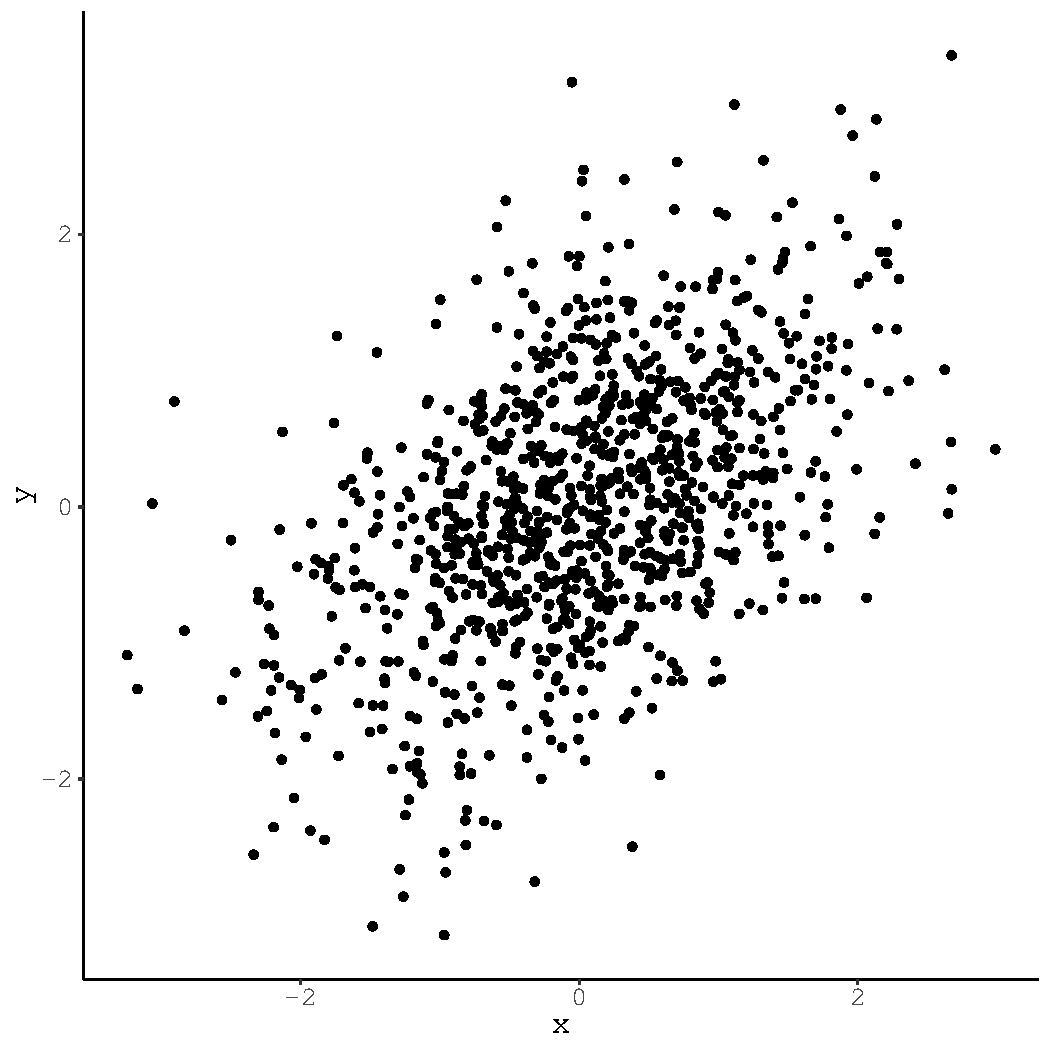
\includegraphics[width=0.9\linewidth]{figure/unnamed-chunk-36-1} 

}



\end{knitrout}
}
\only<2>{
\begin{knitrout}\footnotesize
\definecolor{shadecolor}{rgb}{0.878, 0.918, 0.933}\color{fgcolor}

{\centering 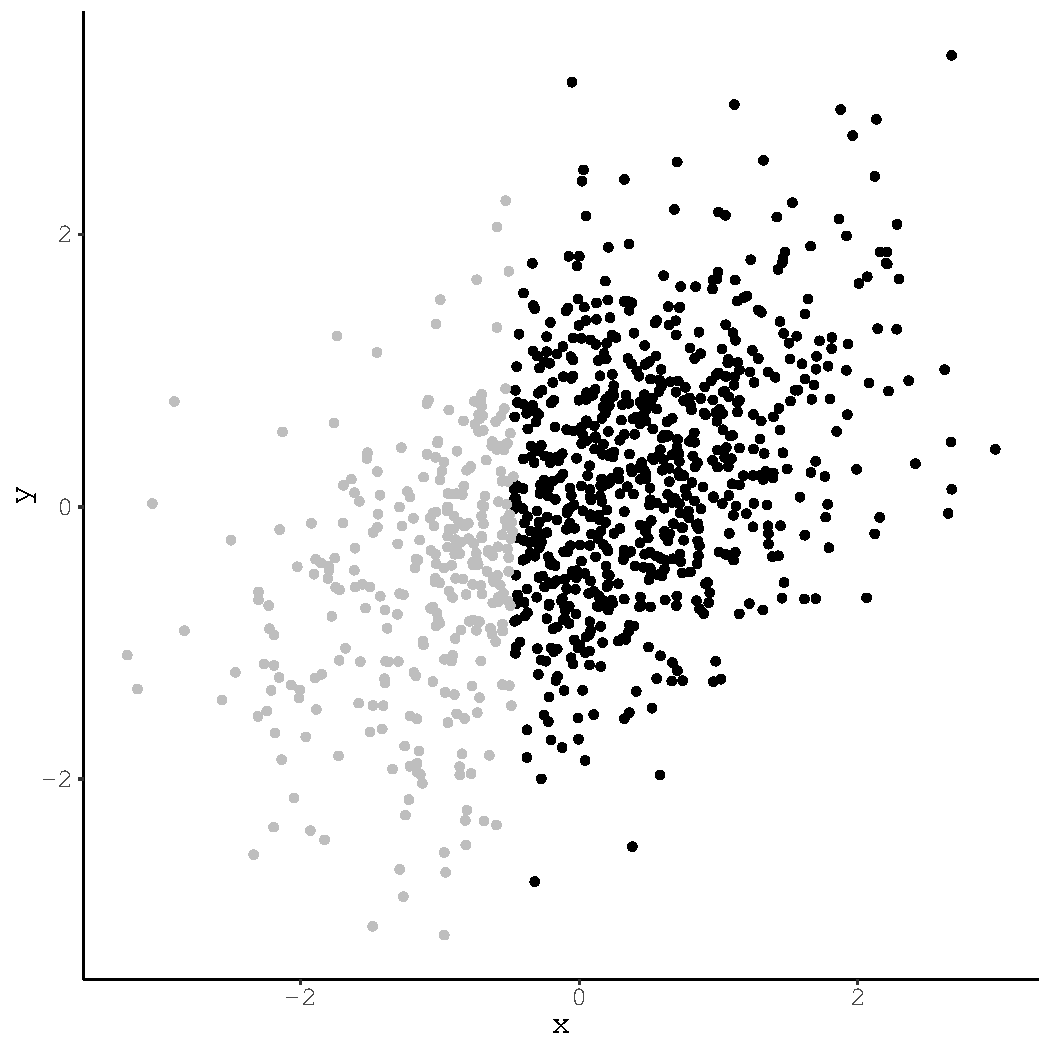
\includegraphics[width=0.9\linewidth]{figure/unnamed-chunk-37-1} 

}



\end{knitrout}
}

\end{column}
\end{columns}
  
\end{frame}

%------------------------------------------------------------------------------%

\begin{frame}[fragile]{Expected Imputation Model Parameters}
   
\begin{columns}
\begin{column}{0.5\textwidth}

\begin{knitrout}\footnotesize
\definecolor{shadecolor}{rgb}{0.878, 0.918, 0.933}\color{fgcolor}\begin{kframe}
\begin{alltt}
\hlstd{lsFit} \hlkwb{<-} \hlkwd{lm}\hlstd{(y} \hlopt{~} \hlstd{x} \hlopt{+} \hlstd{z,}
            \hlkwc{data} \hlstd{= yObs)}

\hlstd{beta}  \hlkwb{<-} \hlkwd{coef}\hlstd{(lsFit)}
\hlstd{sigma} \hlkwb{<-} \hlkwd{summary}\hlstd{(lsFit)}\hlopt{$}\hlstd{sigma}

\hlkwd{as.matrix}\hlstd{(beta)}
\end{alltt}
\begin{verbatim}
##                    [,1]
## (Intercept)  0.04575127
## x            0.49029969
## z           -0.15117793
\end{verbatim}
\begin{alltt}
\hlstd{sigma}
\end{alltt}
\begin{verbatim}
## [1] 0.835231
\end{verbatim}
\end{kframe}
\end{knitrout}

\end{column}
\begin{column}{0.5\textwidth}
    
\begin{knitrout}\footnotesize
\definecolor{shadecolor}{rgb}{0.878, 0.918, 0.933}\color{fgcolor}

{\centering 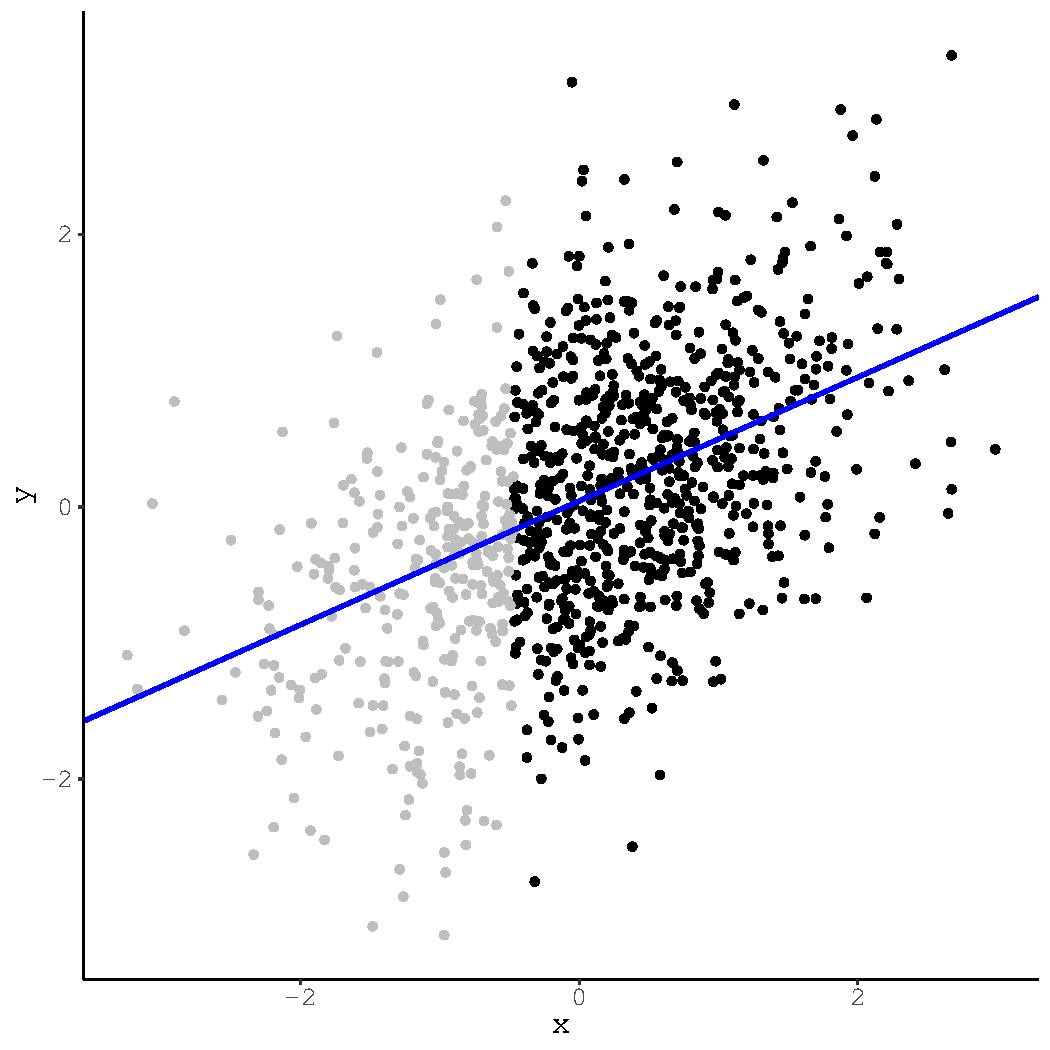
\includegraphics[width=0.9\linewidth]{figure/unnamed-chunk-39-1} 

}



\end{knitrout}
  
\end{column}
\end{columns}

\end{frame}

%------------------------------------------------------------------------------%

\begin{frame}[fragile]{Conditional Mean Substitution}

\begin{columns}
\begin{column}{0.5\textwidth}

\begin{knitrout}\footnotesize
\definecolor{shadecolor}{rgb}{0.878, 0.918, 0.933}\color{fgcolor}\begin{kframe}
\begin{alltt}
\hlcom{## Generate imputations:}
\hlstd{imps} \hlkwb{<-} \hlstd{beta[}\hlnum{1}\hlstd{]} \hlopt{+}
    \hlstd{beta[}\hlnum{2}\hlstd{]} \hlopt{*} \hlstd{yMis[ ,} \hlstr{"x"}\hlstd{]} \hlopt{+}
    \hlstd{beta[}\hlnum{3}\hlstd{]} \hlopt{*} \hlstd{yMis[ ,} \hlstr{"z"}\hlstd{]}

\hlcom{## Fill missing cells in Y:}
\hlstd{dat1[rVec,} \hlstr{"y"}\hlstd{]} \hlkwb{<-} \hlstd{imps}

\hlkwd{round}\hlstd{(}\hlkwd{head}\hlstd{(dat1,} \hlkwc{n} \hlstd{=} \hlnum{5}\hlstd{),} \hlnum{3}\hlstd{)}
\end{alltt}
\begin{verbatim}
##        y      x      z
## 1 -0.339 -0.942 -0.510
## 2  1.123 -0.161 -0.572
## 3  0.302  0.075 -1.980
## 4  0.325  0.850 -0.283
## 5  0.352 -0.400 -1.207
\end{verbatim}
\end{kframe}
\end{knitrout}

\end{column}
\begin{column}{0.5\textwidth}

\begin{knitrout}\footnotesize
\definecolor{shadecolor}{rgb}{0.878, 0.918, 0.933}\color{fgcolor}

{\centering 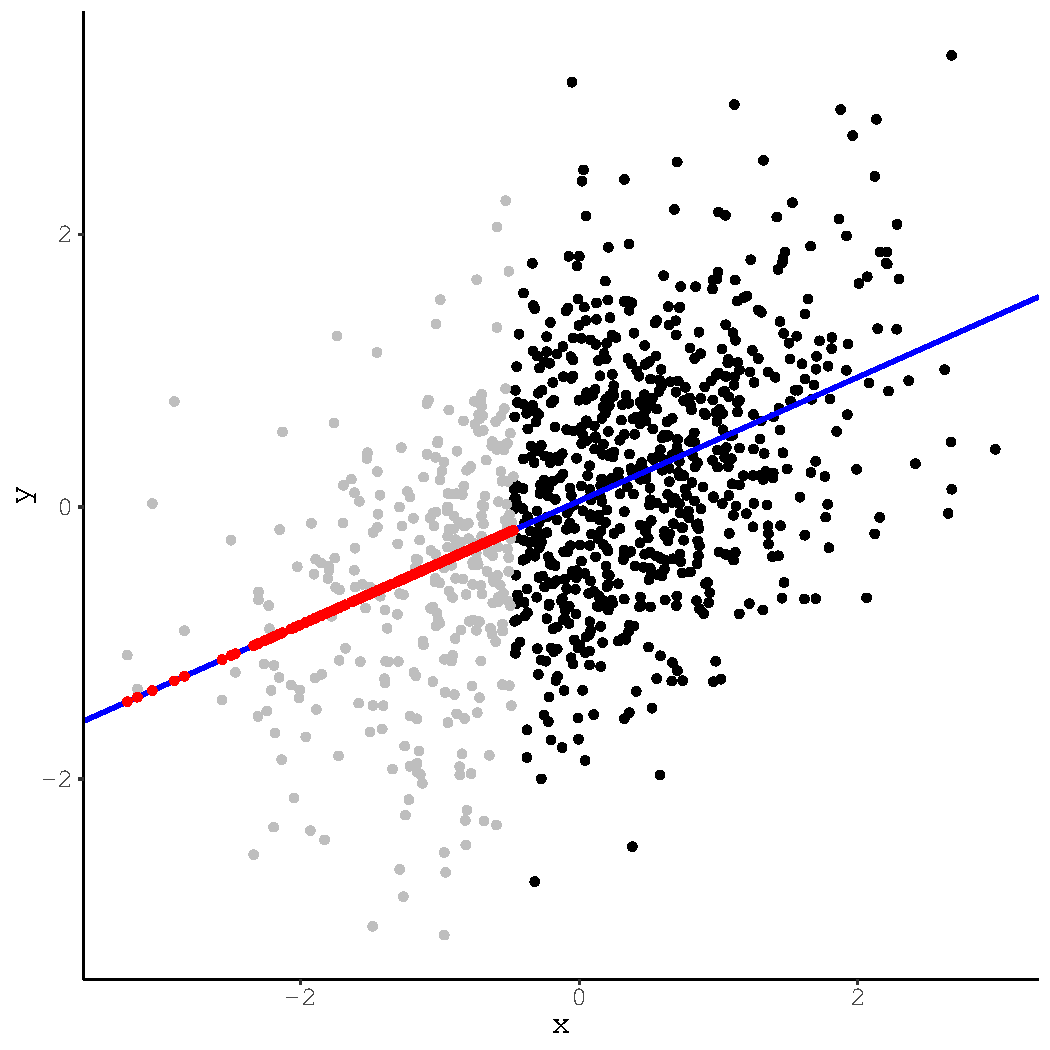
\includegraphics[width=0.9\linewidth]{figure/unnamed-chunk-41-1} 

}



\end{knitrout}
  
\end{column}
\end{columns}

\end{frame}

%------------------------------------------------------------------------------%

\begin{frame}[fragile]{Stochastic Regression Imputation}
   
\begin{columns}
\begin{column}{0.52\textwidth}
  
\begin{knitrout}\footnotesize
\definecolor{shadecolor}{rgb}{0.878, 0.918, 0.933}\color{fgcolor}\begin{kframe}
\begin{alltt}
\hlcom{## Generate imputations:}
\hlstd{imps} \hlkwb{<-} \hlstd{imps} \hlopt{+}
    \hlkwd{rnorm}\hlstd{(}\hlkwd{nrow}\hlstd{(yMis),} \hlnum{0}\hlstd{, sigma)}

\hlcom{## Fill missing cells in Y:}
\hlstd{dat1[rVec,} \hlstr{"y"}\hlstd{]} \hlkwb{<-} \hlstd{imps}

\hlkwd{round}\hlstd{(}\hlkwd{head}\hlstd{(dat1,} \hlkwc{n} \hlstd{=} \hlnum{5}\hlstd{),} \hlnum{3}\hlstd{)}
\end{alltt}
\begin{verbatim}
##       y      x      z
## 1 0.714 -0.942 -0.510
## 2 1.123 -0.161 -0.572
## 3 0.302  0.075 -1.980
## 4 0.325  0.850 -0.283
## 5 0.352 -0.400 -1.207
\end{verbatim}
\end{kframe}
\end{knitrout}

\end{column}
\begin{column}{0.5\textwidth}
  
\begin{knitrout}\footnotesize
\definecolor{shadecolor}{rgb}{0.878, 0.918, 0.933}\color{fgcolor}

{\centering 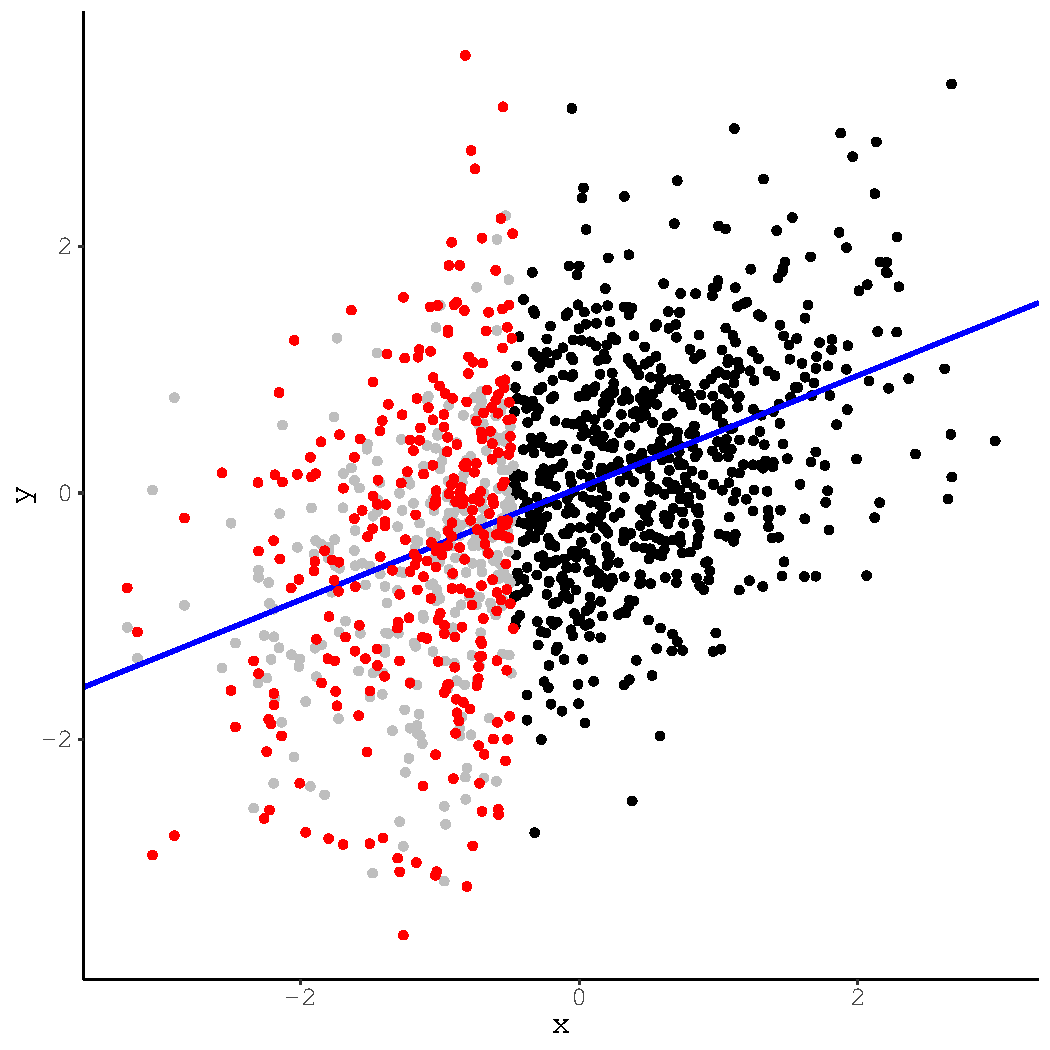
\includegraphics[width=0.9\linewidth]{figure/unnamed-chunk-43-1} 

}



\end{knitrout}
  
\end{column}
\end{columns}

\end{frame}

\watermarkon %-----------------------------------------------------------------%

\begin{frame}{Flavors of MI}
  
  MI simply repeats a single regression imputation $M$ times.
  \begin{itemize}
  \item The specifics of the underlying regression imputation are important.
  \end{itemize}
  \vb
  \pause
  Simply repeating the stochastic regression imputation procedure described 
  above won't suffice.
  \begin{itemize}
  \item Still produces too many Type I errors
  \end {itemize}
  
% latex table generated in R 4.0.2 by xtable 1.8-4 package
% Fri Sep 18 13:27:35 2020
\begin{table}[ht]
\centering
\scalebox{0.8}{
\begin{tabular}{rccc}
  \toprule
 & Complete Data & PN-Type & PNE-Type \\ 
  \midrule
cor(X, Y) & 0.499 & 0.499 & 0.498 \\ 
  Type I Error & 0.040 & 0.066 & 0.046 \\ 
   \bottomrule
\end{tabular}
}
\caption{Mean Correlation Coefficients and Type I Error Rates} 
\end{table}


\vx{-16}
\begin{itemize}
\item Type I error rates for PN-Type MI are much better than they were for 
  single stochastic regression imputation, but they're still too high.
\end{itemize}

\end{frame}

%------------------------------------------------------------------------------%

\begin{frame}{Proper MI}
  
  The problems on the previous slide arise from using the same regression 
  coefficients to create each of the $M$ imputations.
  \begin{itemize}
  \item Implies that you're using the ``correct'' coefficients.
    \vb
  \item This assumption is plainly ridiculous.
    \begin{itemize}
    \item Any estimated regression line is only a guess of the true regression
      line.
      \vc
    \item Hence the standard errors of the coefficients.
    \end{itemize}
    \vb
    \pause
  \item Proper MI also models uncertainty in the regression coefficients used to 
    create the imputations.
    \begin{itemize}
    \item A different set of coefficients is randomly sampled (using Bayesian 
      simulation) to create each of the $M$ imputations.
      \vc
    \item The tricky part about implemented MI is deriving the distributions 
      from which to sample these coefficients.
    \end{itemize}
  \end{itemize}
  
\end{frame}

\watermarkoff %----------------------------------------------------------------%

\begin{frame}{Visualizing MI}
  


Use Bayesian simulation to estimate posterior distributions for the imputation 
model parameters:\\

\vb

\begin{columns}
\begin{column}{0.5\textwidth}

\begin{knitrout}\footnotesize
\definecolor{shadecolor}{rgb}{0.878, 0.918, 0.933}\color{fgcolor}

{\centering 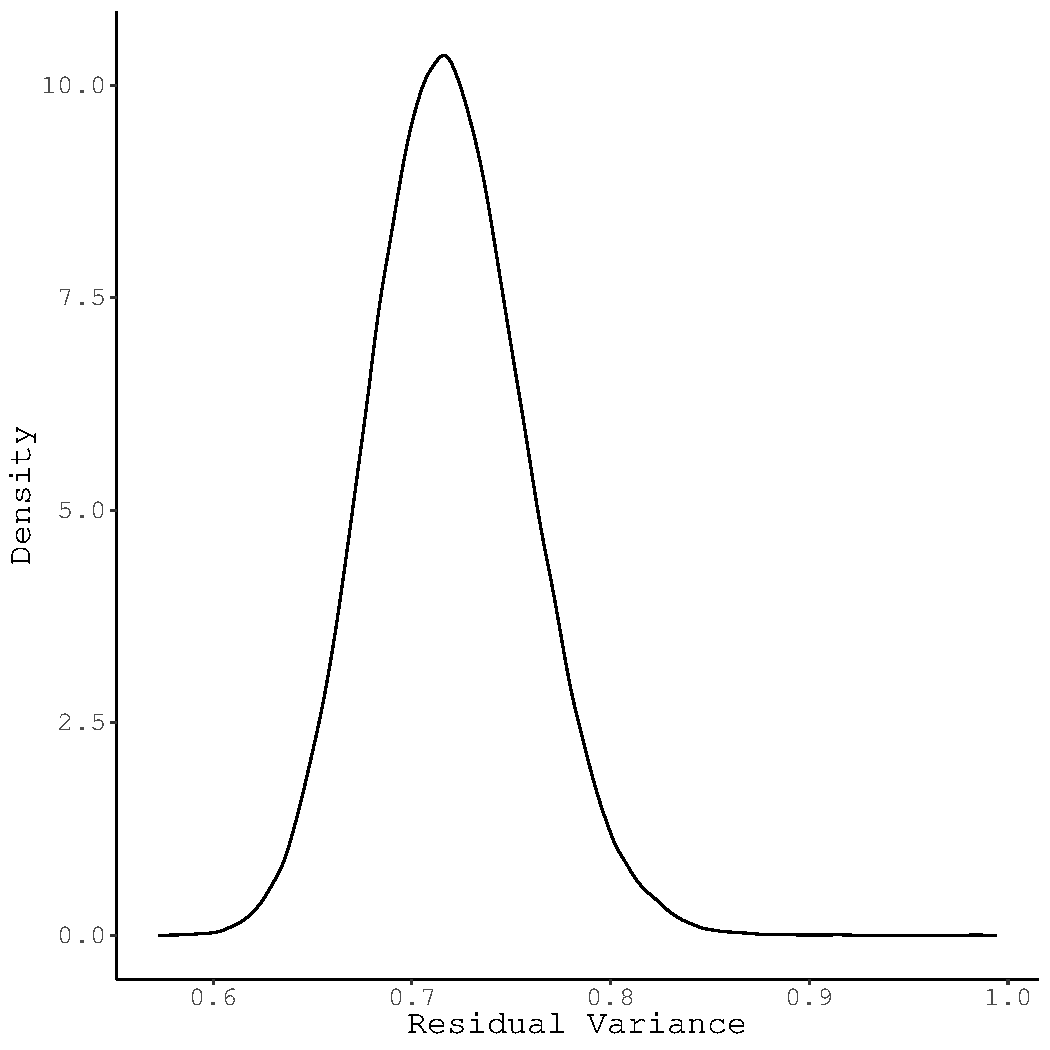
\includegraphics[width=0.9\linewidth]{figure/unnamed-chunk-46-1} 

}



\end{knitrout}

\end{column}
\begin{column}{0.5\textwidth}
  
\begin{knitrout}\footnotesize
\definecolor{shadecolor}{rgb}{0.878, 0.918, 0.933}\color{fgcolor}

{\centering 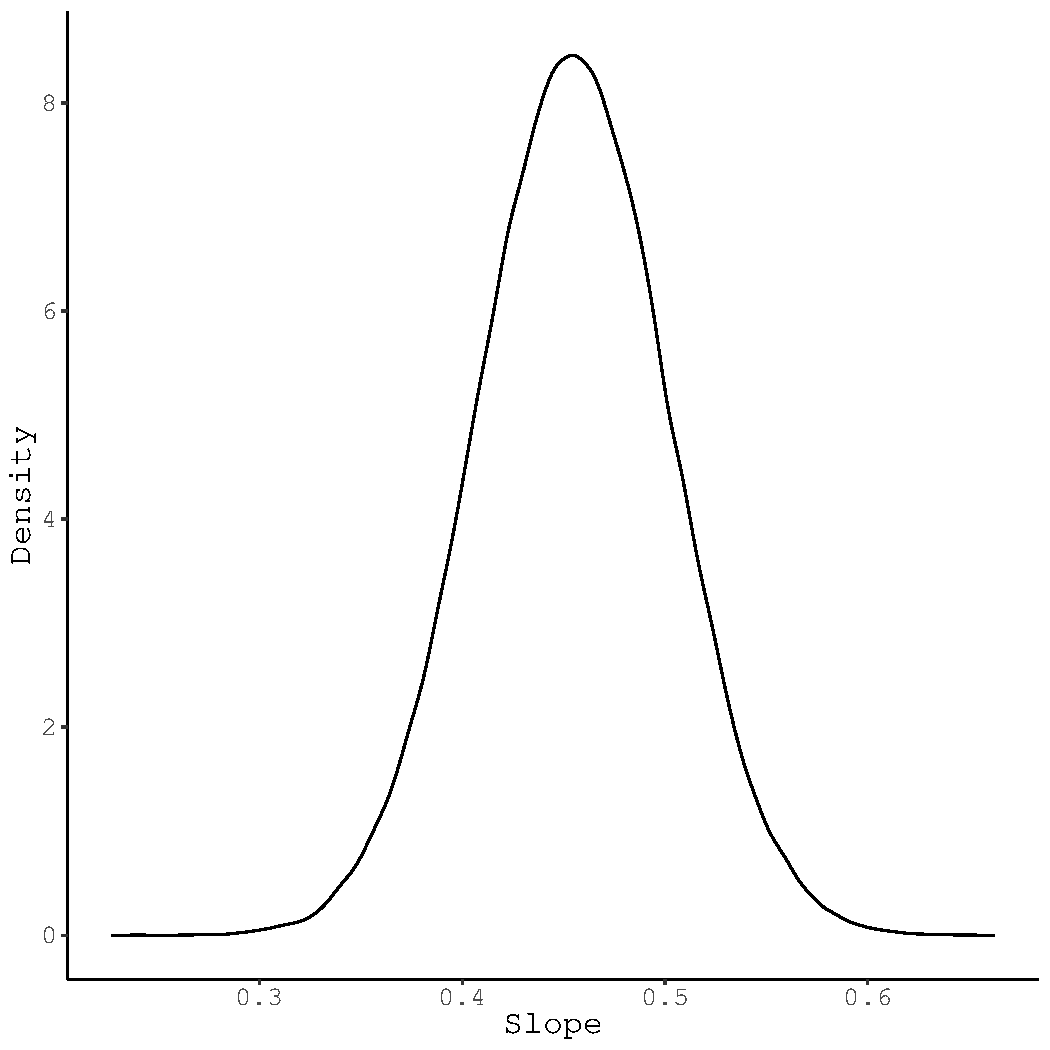
\includegraphics[width=0.9\linewidth]{figure/unnamed-chunk-47-1} 

}



\end{knitrout}

\end{column}
\end{columns}

\end{frame}

%------------------------------------------------------------------------------%

\begin{frame}{Visualizing MI}
  
\begin{columns}
\begin{column}{0.5\textwidth}

  \only<1>{
    Recall the incomplete data.
  }
  
  \only<2>{
    Sample values of $\beta_0$ and $\beta_1$:
    \begin{itemize}
    \item $\beta_0 = 0.086$
    \item $\beta_1 = 0.413$
    \end{itemize}
    \vb
    Define the predicted best-fit line:\\ 
    $\hat{Y}_{mis} = 0.086 + 0.413X_{mis}$
  }
  
  \only<3>{
    Sample a value of $\sigma^2$:
    \begin{itemize}
    \item $\sigma^2 = 0.724$
    \end{itemize}
    \vb
    Generate imputations using the same procedure described in Single Stochastic 
    Regression Imputation:
    \begin{align*}
      Y_{imp} &= \hat{Y}_{mis} + \varepsilon\\
      \varepsilon &\sim \text{N}(0, 0.724)
    \end{align*}
  }
  
  \only<4>{
    Sample values of $\beta_0$ and $\beta_1$:
    \begin{itemize}
    \item $\beta_0 = 0.003$
    \item $\beta_1 = 0.455$
    \end{itemize}
    \vb
    Define the predicted best-fit line:\\ 
    $\hat{Y}_{mis} = 0.003 + 0.455X_{mis}$
  }
  
  \only<5>{
    Sample a value of $\sigma^2$:
    \begin{itemize}
    \item $\sigma^2 = 0.788$
    \end{itemize}
    \vb
    Generate imputations using the same procedure described in Single Stochastic 
    Regression Imputation:
    \begin{align*}
      Y_{imp} &= \hat{Y}_{mis} + \varepsilon\\
      \varepsilon &\sim \text{N}(0, 0.788)
    \end{align*}
  }
  
  \only<6>{
    Sample values of $\beta_0$ and $\beta_1$:
    \begin{itemize}
    \item $\beta_0 = 0.086$
    \item $\beta_1 = 0.384$
    \end{itemize}
    \vb
    Define the predicted best-fit line:\\ 
    $\hat{Y}_{mis} = 0.086 + 0.384X_{mis}$
  }
  
  \only<7>{
    Sample a value of $\sigma^2$:
    \begin{itemize}
    \item $\sigma^2 = 0.716$
    \end{itemize}
    \vb
    Generate imputations using the same procedure described in Single Stochastic 
    Regression Imputation:
    \begin{align*}
      Y_{imp} &= \hat{Y}_{mis} + \varepsilon\\
      \varepsilon &\sim \text{N}(0, 0.716)
    \end{align*}
  }
  
\end{column}
\begin{column}{0.5\textwidth}
  
\only<1>{
\begin{knitrout}\footnotesize
\definecolor{shadecolor}{rgb}{0.878, 0.918, 0.933}\color{fgcolor}

{\centering 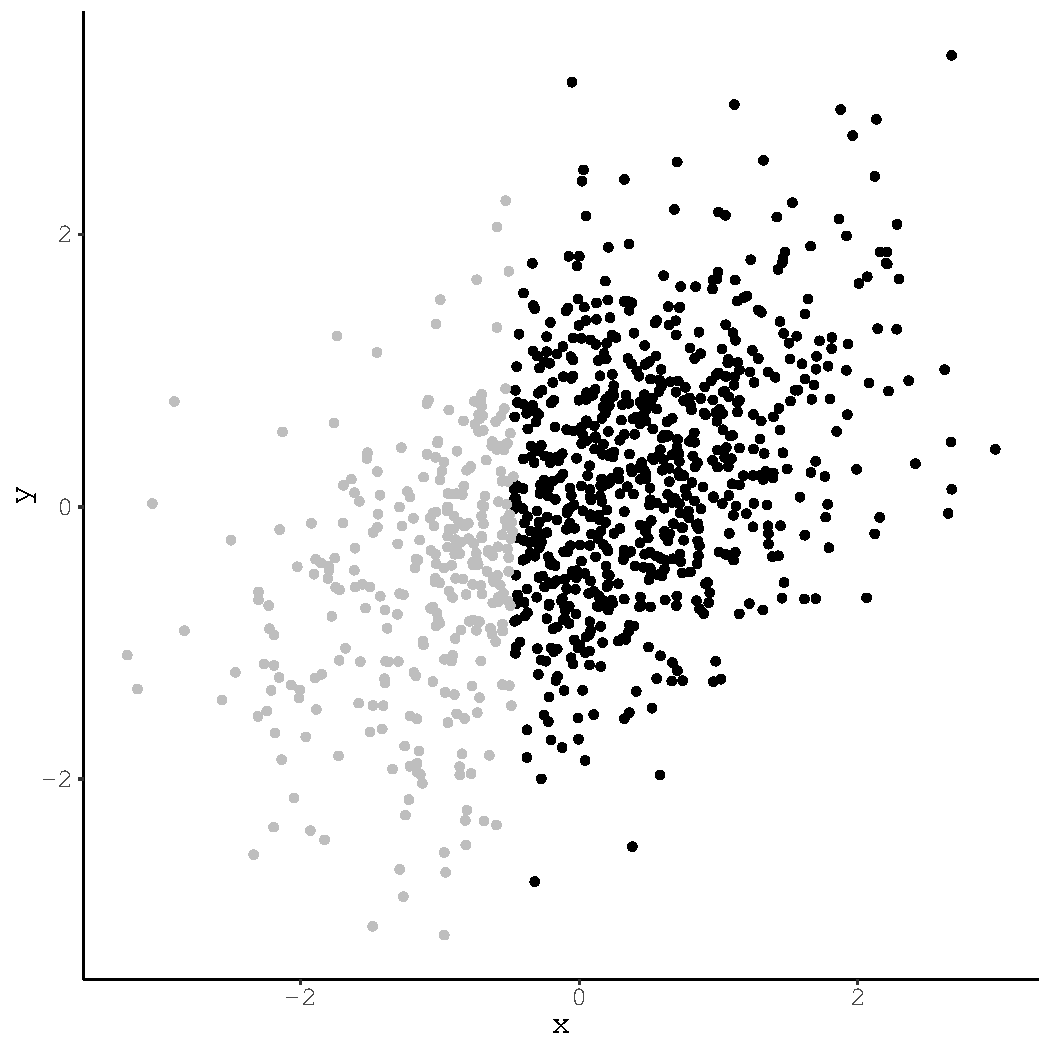
\includegraphics[width=0.9\linewidth]{figure/unnamed-chunk-48-1} 

}



\end{knitrout}
}
\only<2>{
\begin{knitrout}\footnotesize
\definecolor{shadecolor}{rgb}{0.878, 0.918, 0.933}\color{fgcolor}

{\centering 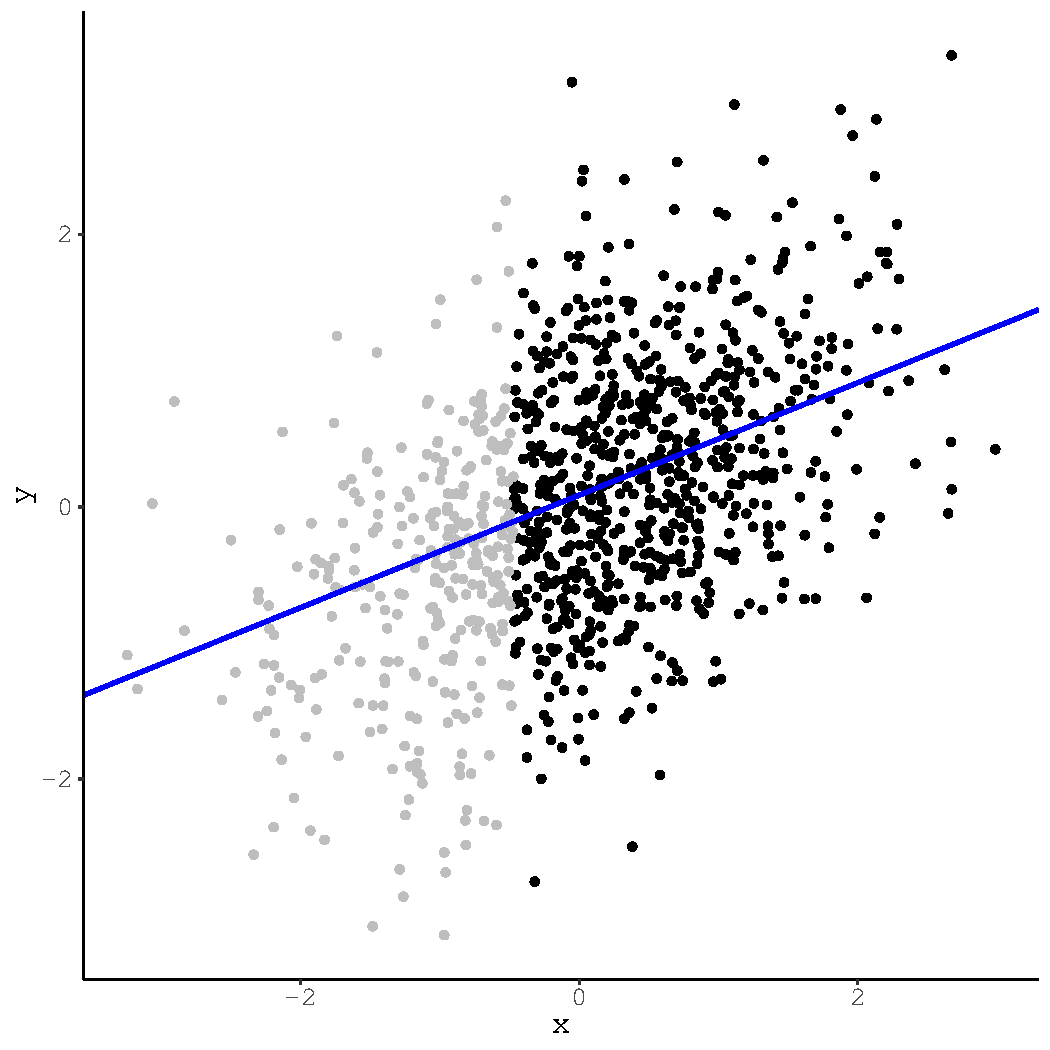
\includegraphics[width=0.9\linewidth]{figure/unnamed-chunk-49-1} 

}



\end{knitrout}
}
\only<3>{
\begin{knitrout}\footnotesize
\definecolor{shadecolor}{rgb}{0.878, 0.918, 0.933}\color{fgcolor}

{\centering 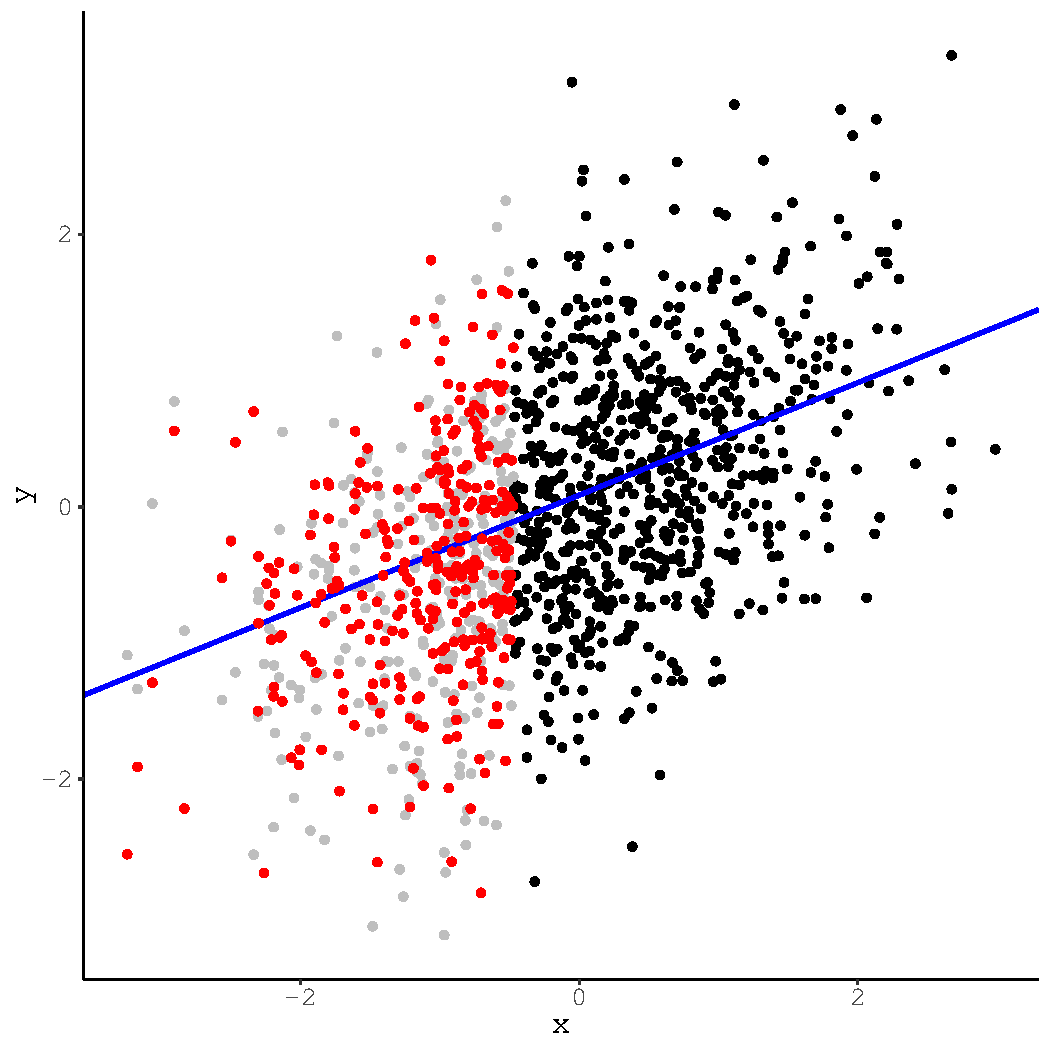
\includegraphics[width=0.9\linewidth]{figure/unnamed-chunk-50-1} 

}



\end{knitrout}
}
\only<4>{
\begin{knitrout}\footnotesize
\definecolor{shadecolor}{rgb}{0.878, 0.918, 0.933}\color{fgcolor}

{\centering 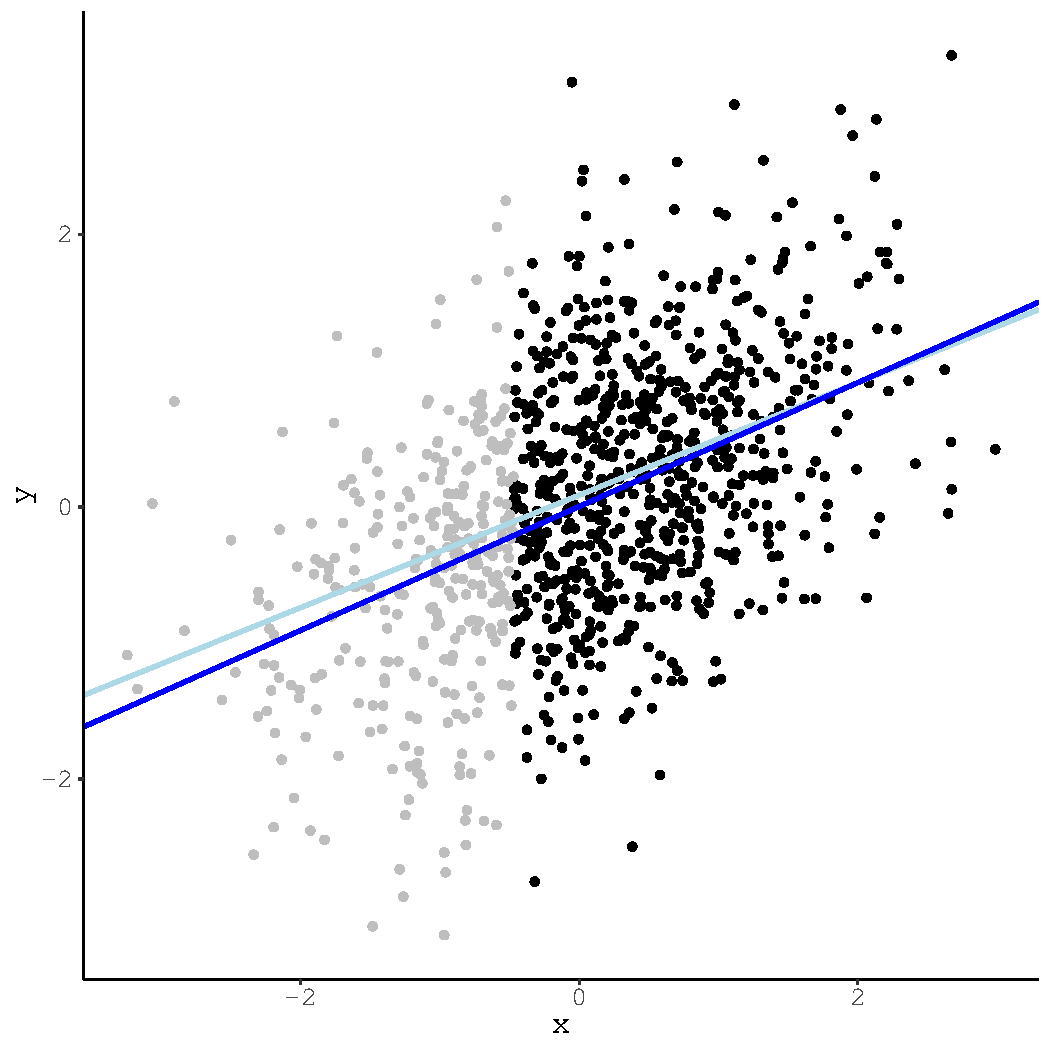
\includegraphics[width=0.9\linewidth]{figure/unnamed-chunk-51-1} 

}



\end{knitrout}
}
\only<5>{
\begin{knitrout}\footnotesize
\definecolor{shadecolor}{rgb}{0.878, 0.918, 0.933}\color{fgcolor}

{\centering 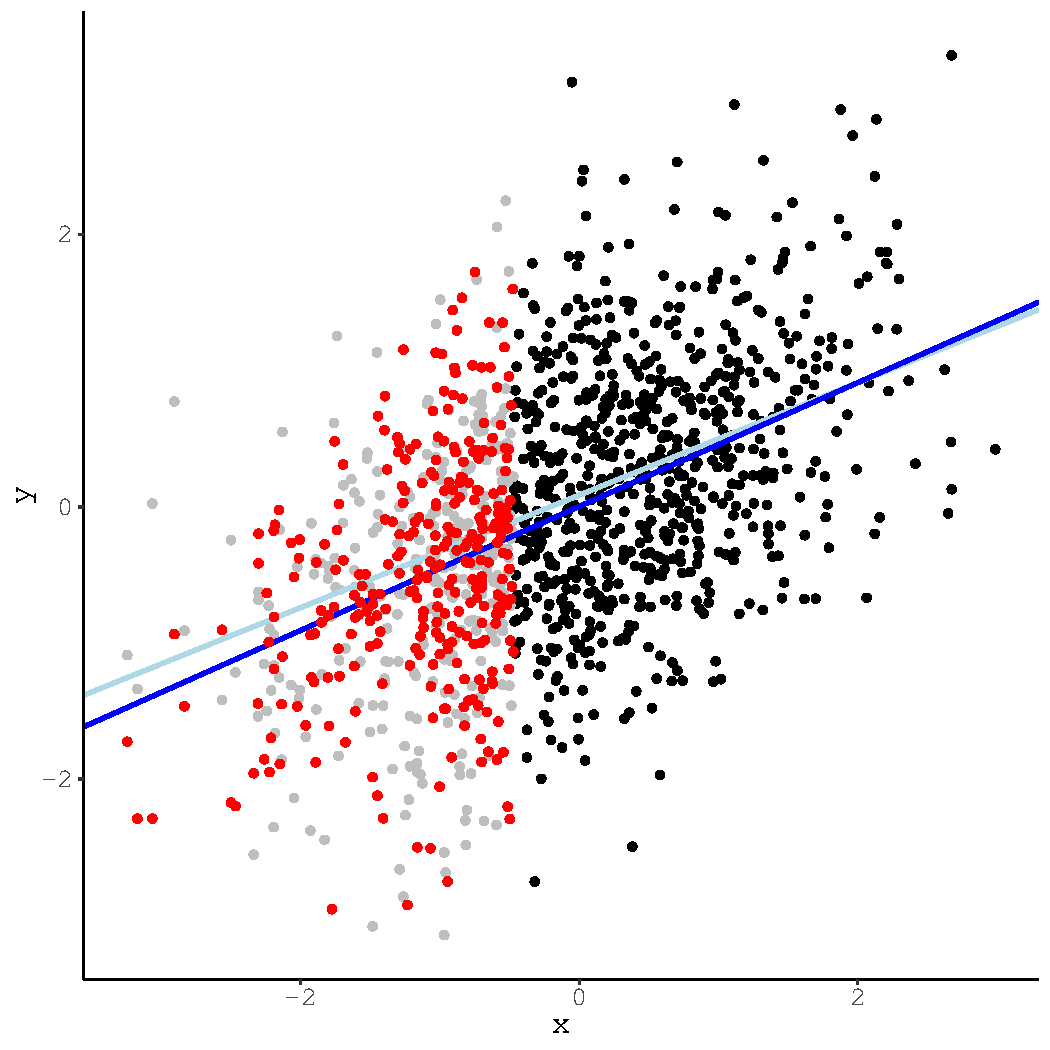
\includegraphics[width=0.9\linewidth]{figure/unnamed-chunk-52-1} 

}



\end{knitrout}
}
\only<6>{
\begin{knitrout}\footnotesize
\definecolor{shadecolor}{rgb}{0.878, 0.918, 0.933}\color{fgcolor}

{\centering 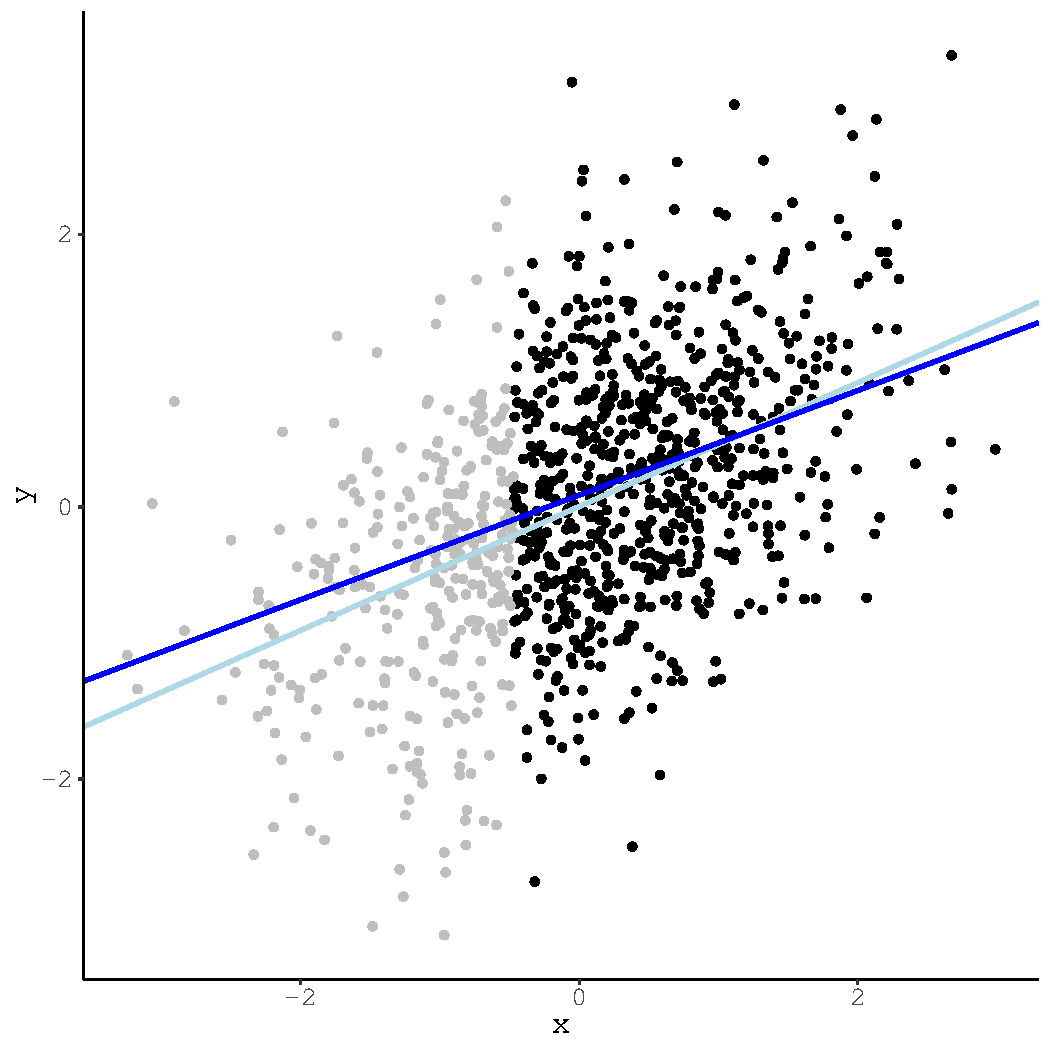
\includegraphics[width=0.9\linewidth]{figure/unnamed-chunk-53-1} 

}



\end{knitrout}
}
\only<7>{
\begin{knitrout}\footnotesize
\definecolor{shadecolor}{rgb}{0.878, 0.918, 0.933}\color{fgcolor}

{\centering 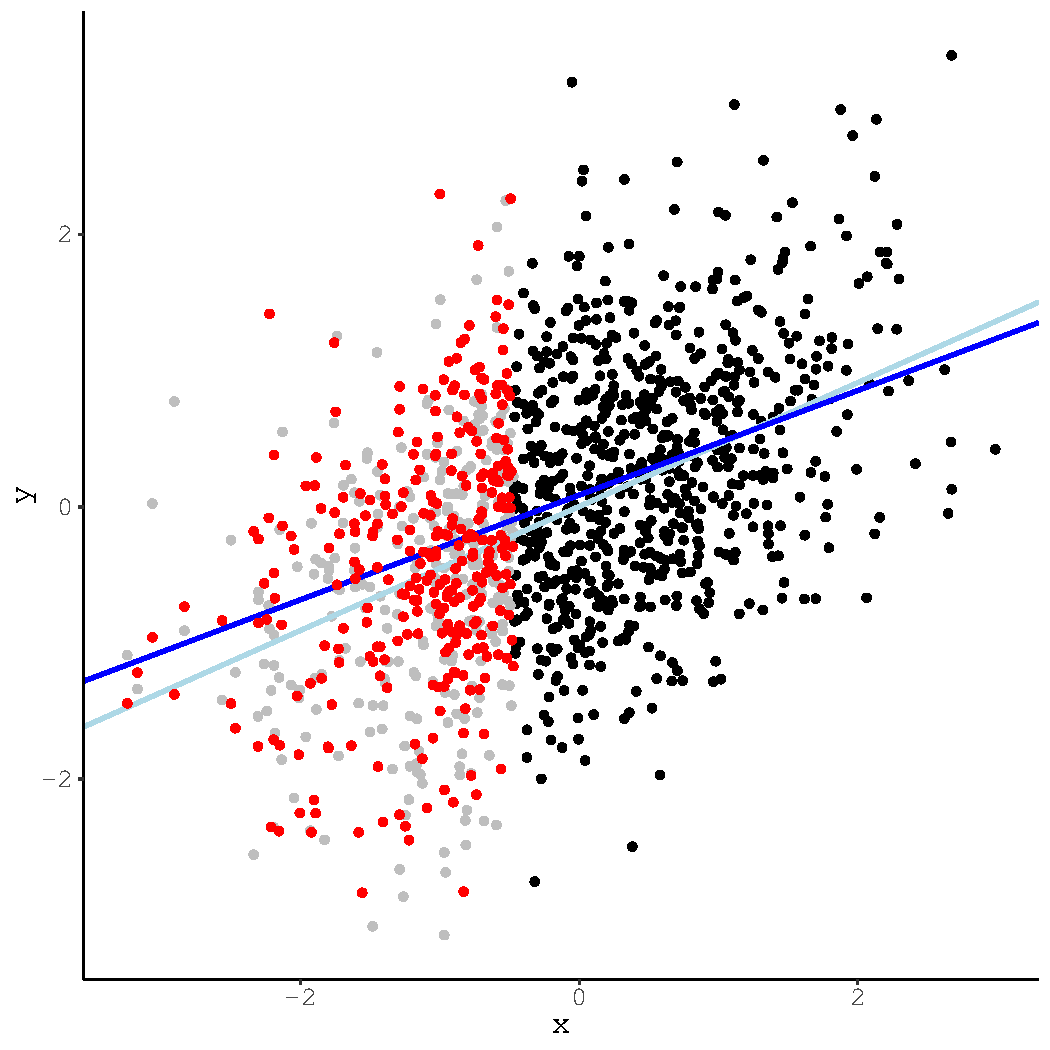
\includegraphics[width=0.9\linewidth]{figure/unnamed-chunk-54-1} 

}



\end{knitrout}
}

\end{column}
\end{columns}

\end{frame}

%------------------------------------------------------------------------------%

\begin{frame}[shrink = 5, fragile]{Doing Imputation in Practice}
  
  Each of the preceding approaches is available in the \textsf{R} package 
  \texttt{mice} \citep{mice}.
  
\begin{knitrout}\footnotesize
\definecolor{shadecolor}{rgb}{0.878, 0.918, 0.933}\color{fgcolor}\begin{kframe}
\begin{alltt}
\hlcom{## Conditional Mean Substitution:}
\hlstd{miceOut1} \hlkwb{<-} \hlkwd{mice}\hlstd{(}\hlkwc{data}   \hlstd{= missData,}
                 \hlkwc{m}      \hlstd{=} \hlnum{1}\hlstd{,}
                 \hlkwc{method} \hlstd{=} \hlstr{"norm.predict"}\hlstd{)}
\hlstd{impDat1} \hlkwb{<-} \hlkwd{complete}\hlstd{(miceOut1)}

\hlcom{## Stochastic Regression Imputation:}
\hlstd{miceOut2} \hlkwb{<-} \hlkwd{mice}\hlstd{(}\hlkwc{data}   \hlstd{= missData,}
                 \hlkwc{m}      \hlstd{=} \hlnum{1}\hlstd{,}
                 \hlkwc{method} \hlstd{=} \hlstr{"norm.nob"}\hlstd{)}
\hlstd{impDat2} \hlkwb{<-} \hlkwd{complete}\hlstd{(miceOut2)}

\hlcom{## Proper MI:}
\hlstd{miceOut3} \hlkwb{<-} \hlkwd{mice}\hlstd{(}\hlkwc{data}   \hlstd{= missData,}
                 \hlkwc{m}      \hlstd{=} \hlnum{25}\hlstd{,}
                 \hlkwc{method} \hlstd{=} \hlstr{"norm"}\hlstd{)}
\hlstd{impList} \hlkwb{<-} \hlkwd{complete}\hlstd{(miceOut3,} \hlstr{"all"}\hlstd{)}
\end{alltt}
\end{kframe}
\end{knitrout}

\end{frame}

\watermarkon %-----------------------------------------------------------------%

\begin{frame}{Doing MI-Based Analysis}
  
  An MI-based data analysis consists of three phases:
  \vb
  \begin{enumerate}
  \item The imputation phase \label{iStep}
    \begin{itemize}
    \item Replace missing values with $M$ plausible estimates.
    \item Produce $M$ completed datasets.
    \end{itemize}
    \vb
  \item The analysis phase \label{aStep}
    \begin{itemize}
    \item Estimate $M$ replicates of your analysis model.
    \item Fit the same model to each of the $M$ datasets from Step \ref{iStep}.
    \end{itemize}
    \vb
  \item The pooling phase
    \begin{itemize}
    \item Combine the $M$ sets of parameter estimates and standard errors from 
      Step \ref{aStep} into a single set of MI estimates.
    \item Use these pooled parameter estimates and standard errors for 
      inference.
    \end{itemize}
  \end{enumerate}
  
\end{frame}

\watermarkoff %----------------------------------------------------------------%

\begin{frame}{Schematic Representation of MI-Bases Analysis}

  \begin{center}
    \includegraphics<1>[width = 0.75\textwidth]{figures/mi_schematic0.pdf}
    \includegraphics<2>[width = 0.75\textwidth]{figures/mi_schematic1.pdf}
    \includegraphics<3>[width = 0.75\textwidth]{figures/mi_schematic2.pdf}
    \includegraphics<4>[width = 0.75\textwidth]{figures/mi_schematic.pdf}
  \end{center}
  
\end{frame}

\watermarkon %-----------------------------------------------------------------%

\begin{frame}{Pooling MI Estimates}
  
  \citet{rubin:1987} formulated a simple set of pooling rules for MI estimates.
  \vb
  \begin{itemize}
  \item The MI point estimate of some interesting quantity, $Q^*$, is simply 
    the mean of the $M$ estimates, $\{\hat{Q}_m\}$:
    \begin{align*}
      Q^* &= \frac{1}{M} \sum_{m = 1}^M \hat{Q}_m\\
    \end{align*}
  \end{itemize}
  
\end{frame}

%------------------------------------------------------------------------------%

\begin{frame}{Pooling MI Estimates}
  
  The MI variability estimate, $T$, is a slightly more complex entity.
  \vb
  \begin{itemize}
  \item A weighted sum of the \emph{within-imputation} variance, $W$, and the 
    \emph{between-imputation} variance, $B$.
    \begin{align*}
      W &= \frac{1}{M} \sum_{m = 1}^M SE(\hat{Q}_m)^2\\
      B &= \frac{1}{M - 1} \sum_{m = 1}^M \left( \hat{Q}_m - Q^* \right)^2\\
      T &= W + \left( 1 + M^{-1} \right) B\\ 
      &= W + B + \frac{B}{M}
    \end{align*}
  \end{itemize}
  
\end{frame}

%------------------------------------------------------------------------------%

\begin{frame}{Inference with MI Estimates}
  
  After computing $Q^*$ and $T$, we combine them in the usual way to get test 
  statistics and confidence intervals.
  \begin{align*}
    t &= \frac{Q^* - Q_0}{\sqrt{T}}\\
    CI &= Q^* \pm t_{crit} \sqrt{T}
  \end{align*}
  
  We must take care with our \emph{df}, though.
  \begin{align*}
    df = (M - 1) \left[1 + \frac{W}{\left(1 + M^{-1}\right)B}\right]^2
  \end{align*}
  
\end{frame}

%------------------------------------------------------------------------------%

\begin{frame}{Fraction of Missing Information}
  
  In Lecture 4, we briefly discussed a very desirable measure of nonresponse: 
  \emph{fraction of missing information} (FMI).
  
  \begin{align*}
    FMI = \frac{r + \frac{2}{(df + 3)}}{r + 1} \approx \frac{(1 + M^{-1})B}{(1 + M^{-1})B + W} \rightarrow \frac{B}{B + W}
  \end{align*}
  where
  \begin{align*}
    r = \frac{(1 + M^{-1})B}{W}
  \end{align*}
  The FMI gives us a sense of how much the missing data (and their treatment) 
  have influenced our parameter estimates.
  \vc
  \begin{itemize}
  \item We should report the FMI for an estimated parameter along with other 
    ancillary statistics (e.g., t-tests, p-values, effect sizes, etc.).
  \end{itemize}
  
\end{frame}

%------------------------------------------------------------------------------%

\begin{frame}[allowframebreaks]{Prediction/Cross-Validation with MI Data}

  When doing an MI-based analysis, we generally want to pool results as late as 
  possible in the analytic process.
  \vc
  \begin{itemize}
  \item This pattern also holds when doing prediction/cross-validation with MI 
    data.
    \vc
  \item When doing prediction, we pool the $M$ sets of predictions.
    \begin{itemize}
    \item We don't generate predictions using the pooled parameters.
    \end{itemize}
    \vc
  \item When doing cross-validation, we pool the $M$ sets of MSE values.
    \begin{itemize}
    \item We don't generate MSE values using pooled predictions or parameters.
    \end{itemize}
  \end{itemize}
  
  \pagebreak
  
  To generate predictions from $M$ multiply imputed datasets, we would:
  \begin{enumerate}
  \item Train the model on each of the $M$ datasets separately.
  \item Generate $M$ sets of predictions from the $M$ models trained above.
  \item Average the $M$ sets of predictions into a single vector of predicted 
    values.
  \end{enumerate}
  \vb
  To run (K-fold) cross-validation with $M$ multiply imputed datasets, we need 
  to:
  \begin{enumerate}
  \item Split each of the $M$ imputed datasets.
  \item Run the cross-validation procedure separately on each of the $M$ imputed 
    datasets.
  \item Pool the final $M$ sets of MSE values.
  \end{enumerate}
  
\end{frame}

%------------------------------------------------------------------------------%

\begin{frame}[allowframebreaks]{Conclusion}
  
  \begin{itemize}
  \item We can use a fitted regression model to generate predictions of new 
    outcomes.
    \vc
  \item We can get two different types of interval estimates around predictions: 
    \emph{confidence intervals} and \emph{prediction intervals}.
    \vc
  \item When building predictive models, we don't care that much about which 
    variables are used.
    \begin{itemize}
    \item We want to get the best possible predictions.
    \end{itemize}
    \vc
  \item When assessing predictive performance, we should consider 
    \emph{test-set} performance, not \emph{training-set} performance.
    \vc
  \item We can use (k-fold) cross-validation to tune our models and estimate 
    prediction error.
    
    \pagebreak
    
  \item Missing data imputation is a very useful type of prediction.
    \vc
  \item We can differentiate between three levels of uncertainty modeling in 
    imputation: \emph{P-}, \emph{PN-}, and \emph{PNE-type}.
    \begin{itemize}
    \item To achieve correct inferences, we need to use full PNE-type multiple 
      imputation.
    \end{itemize}
    \vc
  \item An MI-based analysis consists of three phases: \emph{imputation}, 
    \emph{analysis}, and \emph{pooling}.
    \vc
  \item We should report the FMI for any parameter estimated in an MI-based 
    analysis.
  \end{itemize}
  
\end{frame}

%------------------------------------------------------------------------------%

\begin{frame}[allowframebreaks]{References}
  
  \bibliographystyle{apacite}
  \bibliography{../../../literature/bibtexFiles/statMethRefs.bib,../../../literature/bibtexFiles/dissRefsList.bib}
  
\end{frame}

%------------------------------------------------------------------------------%

\end{document}

